\documentclass[a4paper,10pt]{scrartcl}

% \usepackage[utf8]{inputenc}
% \usepackage[ngerman]{babel}
\usepackage{amsmath}
% \usepackage{mathtools}
% \usepackage{subcaption}
% \usepackage[version=4]{mhchem}
\usepackage{graphicx}
% \usepackage{subfigure}
% \usepackage{lmodern}
\usepackage[left=2.50cm, right=2.50cm, top=3cm, bottom=3cm]{geometry}
% \usepackage{setspace}
\usepackage[locale = DE]{siunitx}
\usepackage{float}
% \usepackage{wrapfig}
%\usepackage{booktabs}
\usepackage{siunitx}
\sisetup{per-mode=fraction}
\sisetup{separate-uncertainty = true}
%\usepackage{placeins}

% \usepackage[bottom]{footmisc}
% \usepackage{csquotes}
\usepackage[style=numeric,backend=bibtex,sorting=none]{biblatex}
\addbibresource{bib.bib}
% \usepackage{mwe}
% \usepackage{hyperref}
% \usepackage{caption}
\usepackage{tabularx}
% \usepackage{makecell}


% \usepackage{subfig}
% \usepackage{cleveref}

\addtokomafont{sectioning}{\rmfamily}



\begin{document}
\begin{center}
    \begin{huge}
        \textsc{Technical University of Munich}
    \end{huge}\\

    \vspace{2cm}

    \begin{Large}
        \textsc{Bachelor Thesis}
    \end{Large}\\

    \vspace{2cm}

    \par\noindent\rule{\textwidth}{0.2pt}
    % \vspace{0.5cm}
    \begin{huge}
        \textbf{Improving the Neutrino Oscillation\\}
    \end{huge}
    \vspace{0.1cm}
    \begin{huge}
        \textbf{Sensitivity of IceCube\\}
    \end{huge}
    \vspace{0.3cm}
    \begin{huge}
        \textbf{with Graph Neural Networks}
    \end{huge}
    % \vspace{0.5cm}
    \par\noindent\rule{\textwidth}{0.2pt}

    \vspace{2cm}

    A thesis submitted in fulfillment of the requirements for the degree of BSc Physics

    \vspace{2cm}

    \begin{large}
        Author: Tim Guggenmos\\
        \vspace{0.1cm}
        Supervisors: Elisa Resconi, Rasmus Ørsøe
    \end{large}

    \vspace*{\fill}

    \begin{large}
        September 23, 2022
    \end{large}

\end{center}

\thispagestyle{empty}
\newpage

% \begin{spacing}{1.3}
\tableofcontents
% \end{spacing}

\newpage


% \section{Abstract}

\section{Introduction}

The IceCube Neutrino Observatory is the largest neutrino experiment ever constructed.
It consists of over 5000 light-detecting digital optical modules (DOMs), which are buried in a volume of over \SI{1}{km^3} in the ice of Antarctica.
Such an experiment with as many individual detectors naturally yields tons of raw data, hence manual interpretation/analysis is not appropriate.
One way to analyze the data is the use of Machine Learning (ML) models, more specifically in our case the use of Graph Neural Networks (GNN).
The network relevant to this work models the triggered detectors, as point clouds which are then connected and turned into a graph representing the geometry and data gained from the measurement.
The data fed to the network for interpretation/evaluation includes the measurements and positions of the detectors, as well as the time of measurement.
In this thesis, an effort is made to feed additional data to the network, which describes the local properties of the ice, to help the network understand the data context better.
By also focusing the network's attention on energies most relevant to neutrino oscillations, its performance will be increased in predicting the values necessary to build a mathematical model of neutrino oscillations.

\section{Neutrinos}

Search for the building blocks of matter has long been an interesting field for many scientists and philosophers.
For a long time, humans believed elements to be fundamentally different from one another.
Not too long ago, in the late 1800s-1900s, it was discovered that matter is made from atoms, which in turn consist of protons, neutrons, and electrons.
The idea that these, long thought of as elementary particles, are dividable even further into quarks has not even been around for more than 60 years at the time this work is written.

% \subsection{Standard Model}

The Standard Model of particle physics (shown in figure \ref{fig:standardmodel}) is a theory to describe all currently known elementary particles.
It also describes three of the four fundamental forces we have yet discovered, them being electromagnetic, weak, and strong interactions, with gravity being the force that is not (yet, hopefully) able to be integrated consistently into the theory.

Although the Standard Model explains most phenomena fully and logically, gravity, dark matter, as well as a few other phenomena, are not able to be properly explained/modeled by the Standard Model.
The model is a great achievement of science, and new particles continue to be discovered by great scientists to this day.
But the weaknesses of it mark the theory as incomplete.

\begin{figure}[h]
    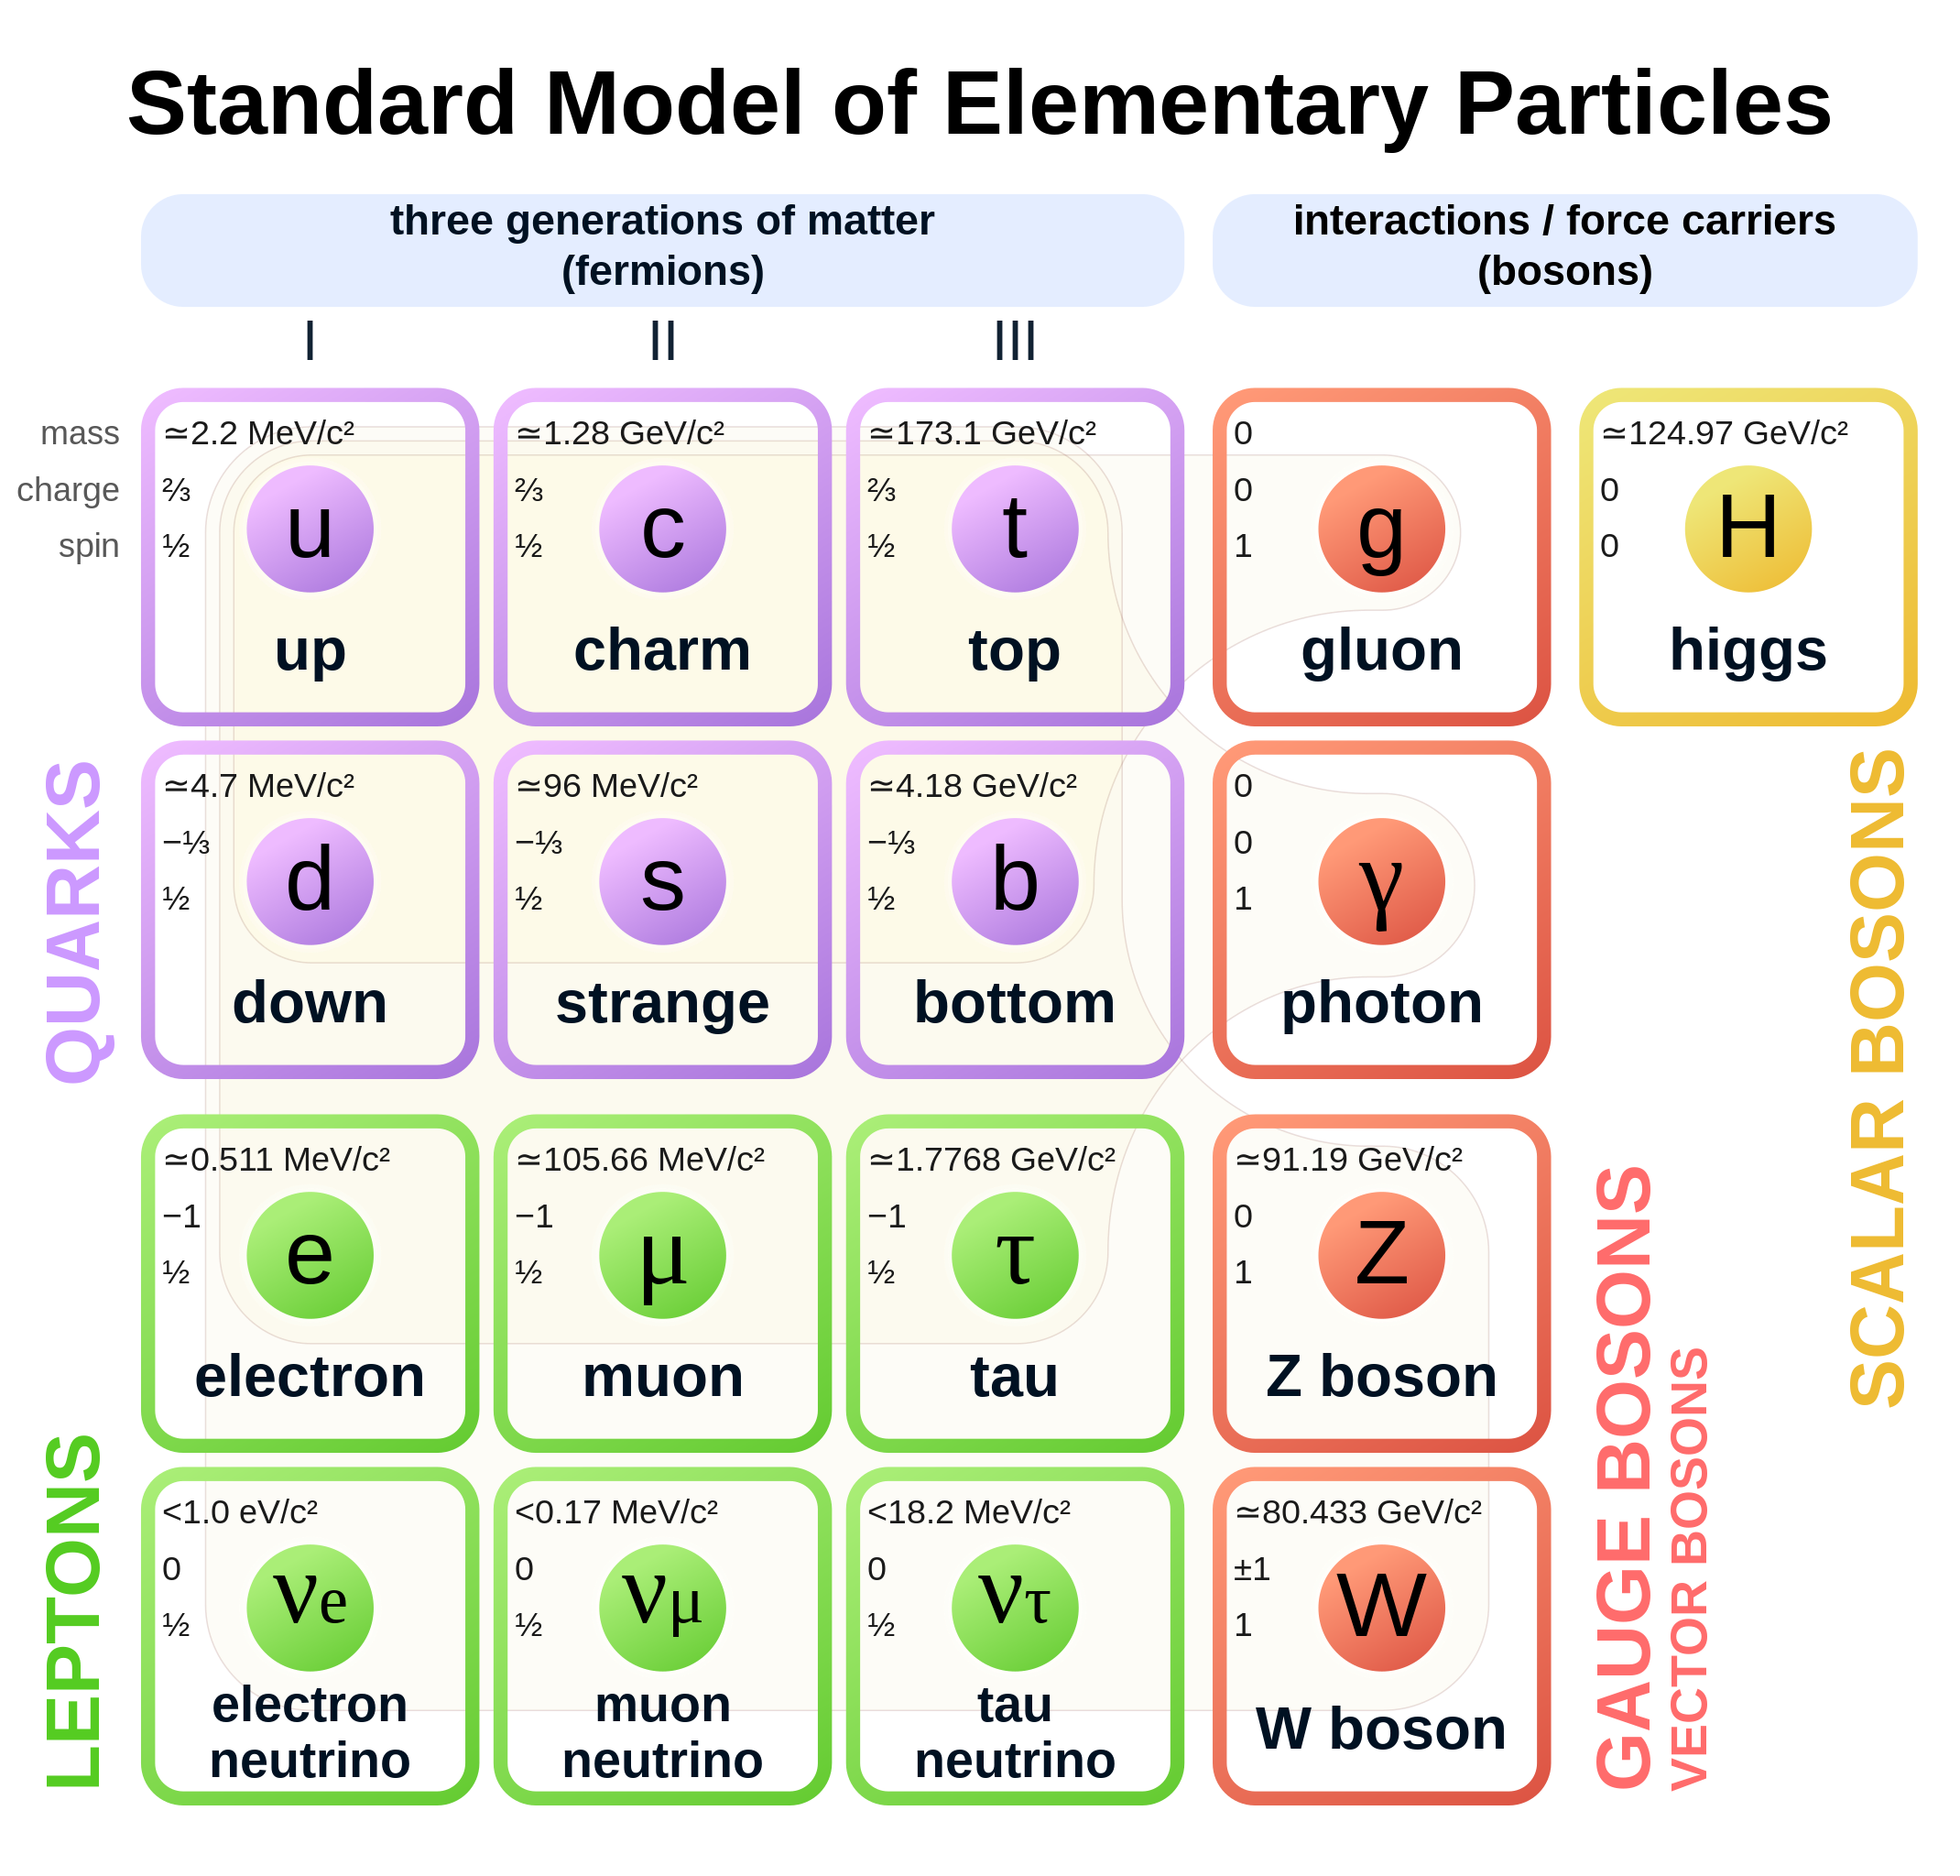
\includegraphics[scale=0.12]{images/Standard_Model_of_Elementary_Particles.svg.png}
    \centering
    \caption{The Standard Model of particle physics \cite{wiki:Standard_Model}.}
    \label{fig:standardmodel}
\end{figure}

% \subsection{Neutrinos}
\label{neutrinos}

Neutrinos, shown at the bottom of the Standard Model above, are uncharged leptons first hypothesized by Wolfgang Pauli in 1930 to fix the observed possible variation of electron energy during beta decay.
He reasoned, that since energy must be conserved, the 'missing' energy is carried by a particle previously not detected/thought of by anyone.

\begin{equation}
    n^0 \longrightarrow p^+ + e^-
\end{equation}

Therefore he extended the known equation of the beta decay (above) with his new electron neutrino particle, which solved the until then continuous beta decay spectrum.

\begin{equation}
    n^0 \longrightarrow p^+ + e^- + \bar{\nu}_e^0
\end{equation}

Since neutrinos exist everywhere in huge numbers, this raises the question of why they have not been detected before.
This is due to them interacting only via the weak force over short distances (as well as gravity), which makes them very hard to detect.
With an estimated cross section of $\sigma \sim \SI{e-38}{cm^2} = \SI{e-42}{m^2}$ their probability of interaction is very small.
For comparison, the standard unit for cross-sections in particle physics, the \texttt{barn}, equals $\SI{1}{b} = \SI{100}{fm^2} = \SI{e-28}{m^2}$.

% As an illustration of how tiny this cross-section is, we will calculate the mean free path $\lambda$ of a neutrino traveling through pure lead (density $\rho = \SI{3.3e22}{cm^{-3}}$).

% \begin{equation}
%     \lambda_{Lead} = \frac{1}{\sigma_{Neutrino} \cdot \rho_{Lead}} = \SI{x}{ly}
% \end{equation}

Because of their low interaction probability and resulting high penetration neutrinos carry information about events throughout the universe.
Observing them may lead to insight and understanding of what happened a long time ago in a galaxy far, far away....

\subsection{Neutrino Oscillation}

In the 1960s the solar neutrino flux was measured in the Homestake experiment performed by Ray Davis and John N. Bahcall.
They measured the number of neutrinos interacting inside a \SI{380}{m^3} tank of perchloroethylene.
The solar neutrinos originate from the nuclear fusion process, mostly from the pp-chain (proton-proton).

\begin{equation}
    p^+ + p^+ \longrightarrow {^2H} + e^+ + \nu_e
\end{equation}

The observed neutrino flux was only about $\frac{1}{3}$ of the theoretically expected value \cite{nbi-neutrino}.
This problem puzzled scientists for decades until it was resolved around 2002 through the explanation of neutrino oscillation.
Neutrino oscillation is a flavor transition of the neutrino, where any neutrino given will oscillate/change its flavor (electron, muon, tau) when traveling through space.
Therefore statistically only about every third neutrino will be an electron neutrino, and only those are being measured by the Homestake experiment - explaining the measured flux deficit.

The three neutrino flavors carry different masses, therefore they travel through space with different velocities.
The actual weight of any neutrino is a superposition (linear combination) of the three individual mass eigenstates.

Because the different neutrino mass states travel through space at different rates, a phase shift is introduced as the neutrino travels.
This results in a pure electron neutrino gaining some mixture of mu and tau neutrino as well.
As each mass state is periodic, after some distance the neutrino will periodically return to its pure electron form, as long as the states maintain coherence.
If coherence is reduced, the neutrino will consist increasingly of an equal mixture of all states, therefore the Solar Neutrino Problem is solved.

The mixing of neutrino states can be described by the following Pontecorvo-Maka-Nakagawa-Sakata (PMNS) matrix.

\begin{equation}
    \begin{bmatrix}
        \nu_{e}   \\
        \nu_{\mu} \\
        \nu_{\tau}
    \end{bmatrix}
    =
    U
    \begin{bmatrix}
        \nu_{1} \\
        \nu_{2} \\
        \nu_{3}
    \end{bmatrix}
    =
    \begin{bmatrix}
        U_{e 1}    & U_{e 2}    & U_{e 3}    \\
        U_{\mu 1}  & U_{\mu 2}  & U_{\mu 3}  \\
        U_{\tau 1} & U_{\tau 2} & U_{\tau 3}
    \end{bmatrix}
    \begin{bmatrix}
        \nu_{1} \\
        \nu_{2} \\
        \nu_{3}
    \end{bmatrix}
\end{equation}

The superposition state of a neutrino can also be described by the mixing angles $\theta_{ij}$ between any two states $i$ and $j$.
In this case, the PMNS matrix can be expressed by three separate rotation matrices containing the mixing angles \cite{warwick}, a math conversion that lies beyond the scope of this work.

% \subsection{Cosmic Rays}

\subsection{Charged/Neutral Current Decays}

As touched on earlier, neutrinos interact in two distinct ways, gravity and the weak force.
The neutrino takes part in two weak interaction types, charged current and neutral current interactions.
The charged current interaction is mediated by the W-boson and allows for interaction with a charged particle.
The Z-boson on the other hand allows for interaction with neutral particles and only affects the spin and momentum of the particles involved.

\begin{figure}[h]
    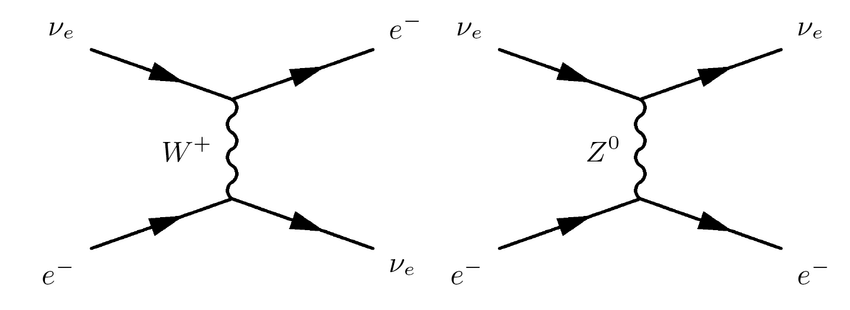
\includegraphics[scale=0.3]{images/charged-and-neutral-current.png}
    \centering
    \caption{Feynman diagrams of charged and neutral current interactions.}
    \label{fig:cc-nc}
\end{figure}


\subsection{Cherenkov Radiation}

The detectors (DOMs) within IceCube can not measure incoming neutrinos directly, instead, they detect radiation that was produced in neutrino interactions.
This electromagnetic radiation is emitted when a charged particle is moving through a dielectric medium at a speed greater than its phase velocity (speed of light within the medium).
This phenomenon is most familiar for its occurrence in nuclear reactors, which glow blue because of emitted beta particles that travel faster than the speed of light in water.

\begin{equation}
    c_{Water} = \frac{c_{Vacuum}}{n_{Water}} = \frac{\SI{3e8}{\frac{m}{s}}}{1.3} = \SI{2.25e8}{\frac{m}{s}}
\end{equation}

When a charged particle travels through a dielectric medium it polarizes the surrounding molecules.
After the charged particle has passed the molecules rearrange themselves into their original orientation.
This change in charge distribution causes electromagnetic radiation known as Cherenkov Radiation.
In case the incoming particle travels faster than the speed of light within the medium, a wavefront is created trailing the particle, similar to a sonic boom (see figure \ref{fig:cherenkovlight}).

\begin{figure}[h]
    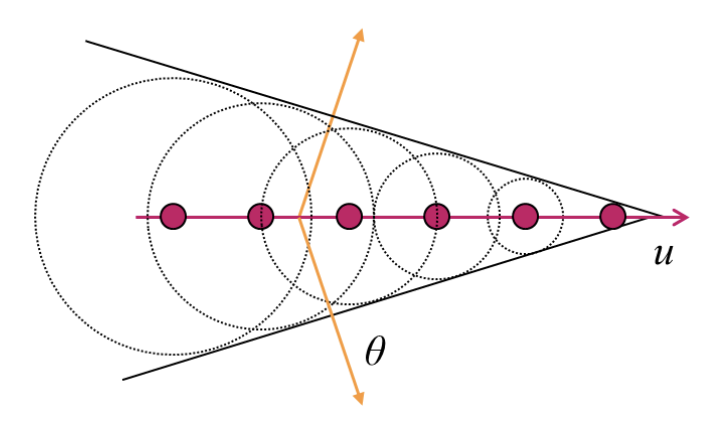
\includegraphics[scale=0.7]{images/cherenkov-light.png}
    \centering
    \caption{An illustration representing a Cherenkov Radiation wavefront \cite{left}.}
    \label{fig:cherenkovlight}
\end{figure}


\section{IceCube}

\subsection{Location and Structure}

The IceCube Neutrino Observatory is located at the geographic South Pole, where it makes use of the abundance of natural ice as material for the incoming particles to interact with.
Over a volume of over \SI{1}{km^3} 5160 Digital Optical Modules (DOMs) have been placed over a span of about 10 years.
The DOMs are positioned on 86 individual strings in a hexagonal grid pattern at depths between \SI{1450}{m} and \SI{2450}{m} (shown in figure \ref{fig:icecube}).
The strings are placed about \SI{125}{m} apart horizontally and all DOMs are spaced about \SI{17}{m} vertically.
Each DOM contains a \SI{10}{"} Photomultiplier Tube (PMT) that faces downwards, towards the bedrock below the ice.
In the center of the detector, where the ice is clearest, additional strings have been placed, which increases the detector density in that volume (DeepCore) \cite{icecube}.

The detector was built to study neutrino and muon interactions with energies between singular GeV up to a few PeV.
It was built so large, not only to increase the probability of a neutrino interaction within its borders, which is minimal (see section \ref{neutrinos}).
But also to provide enough space to hopefully capture full traces of interactions, which can extend up to a few hundred meters in length, especially interactions with high energies that can involve over 100 DOMs.

\subsection{Working Principle}
\label{working-principle}

The neutrino interaction with the ice produces charged particles, which in turn emit Cherenkov radiation when interacting with the ice.
This near-UV radiation is then recorded by the PMTs and registered as a pulse of Cherenkov radiation.

However, not all DOM triggers are caused by a neutrino interaction.
Radioactive decay, as well as the noise of the electronic components are also recorded ($> \SI{1000}{Hz}$).
These events are of course not desired, and many ways of filtering have been implemented to combat such noise in the recorded data \cite{rasmus-master}.

At trigger level, a minimum number of DOMs have to be triggered for them to be registered as a single event.
These triggers have to occur within a specified time interval (8 DOMs within \SI{5}{\mu s}), for them to be counted towards one event.
This tries to ensure that an event does not solely consist of multiple noise hits.

Additionally, local filtering is applied to all events, it filters for triggers that happen close by (\SI{150}{m} radius with a given time frame of \SI{1000}{ns}).
This assures that all DOMs registered as a single event are locally correlated and therefore most likely to be caused by a single neutrino interaction.
For example, a single noise-influenced DOM at the outside of the detector is not included in an actual event at the center of the detector.

\begin{figure}[h]
    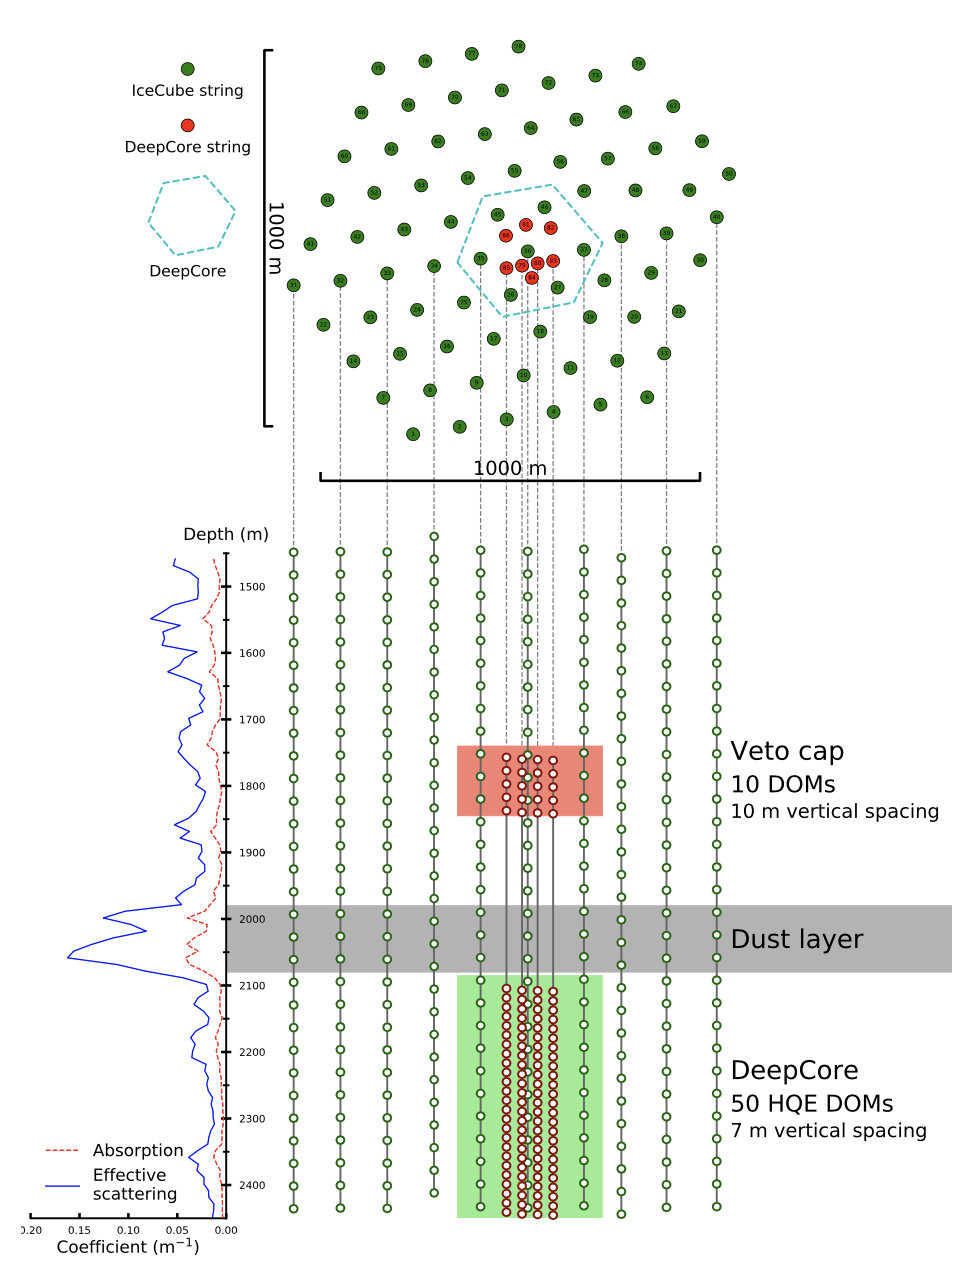
\includegraphics[scale=0.6]{images/icecube.png}
    \centering
    \caption{The structure of IceCube \cite{left}.}
    \label{fig:icecube}
\end{figure}

\subsection{Ice Variance}

The ice on the south pole has been a subject of study since it contains many irregularities.
These irregularities influence the measurements of IceCube in various ways.
The propagation of light depends highly on the optical properties of the ice, the detector medium itself is a source of systematic uncertainties.
For example, a high concentration of dust at a depth of around \SI{2000}{m} (dust layer) results in a higher absorption rate than elsewhere in the detector.
Besides absorption rate, the amount of scattering and birefringence (as well as other properties) vary over the volume, since they were formed at different times, with inconsistent densities and temperatures.

This work will incorporate measurements of ice properties measured by the SPICE project (see section \ref{icedata}) \cite{1301.5361} into the learning process of a neural network (see section \ref{ml} and \ref{graphnet}) to try to help it understand the influence of the ice on neutrino events and improve its performance.

\subsection{Retro}

The most commonly used algorithm for reconstructing low-energy events in IceCube is Retro (Retro Reco) \cite{retro}.
Retro reconstructs events by simulating photons traveling through the ice between DOMs and builds lookup tables mapping simulated physics to observed DOM detections.
By comparing a recorded event to these tables and looking for the entries that are most likely to have occurred (the entries that have the highest agreement between them), it predicts the values of the event.

Since Retro provides great accuracy and is widely used within IceCube, it will serve as a baseline for comparisons later in this work.

\subsection{Simulation Data}

As will be apparent in section \ref{supervised-learning}, it will be necessary for the process of this work to have labeled data of IceCube neutrino events.
That is, having a dataset with not only the event recorded by IceCube but also the true information of the particle it came from.
As this information is of course not known for recorded events (this is what we want to know in the first place), simulated data is used.

The used datasets are generated by \texttt{Genie}, a state-of-the-art neutrino simulation engine.
It provides the most physically accurate data accessible because it simulates neutrino interactions with all ice molecules.

As briefly mentioned above, all datasets used in this work are highly processed, many levels of filtering have been applied to filter out noise in the measuring electronics, and other undesired events.
The level of filtering is described as ''Level 7'' \cite{rasmus-master} and is the highest level of cleaning generally available.
Therefore further mention of noise or other events has to be made.

\subsection{Event Variables}
\label{variables}

For each recorded event, IceCube produces a set of data consisting of the measurements each DOMs participating in that event has made.
This is the data that is available for real recorded events, as well as for simulated data.
The following table will outline the variables \cite{graphnet} generated by each DOM and will serve as input for the Neural Network introduced in section \ref{graphnet}.

\begin{center}
    \begin{tabular}{ |l|l| }
        \hline
        Variable Name & Description                 \\
        \hline
        dom\_x        & X coordinate of the DOM     \\
        dom\_y        & Y coordinate of the DOM     \\
        dom\_z        & Z coordinate of the DOM     \\
        dom\_time     & Time the DOM was triggered  \\
        dom\_charge   & Charge the DOM measured     \\
        rqe           & Relative quantum efficiency \\
        pulse\_width  & Width of the pulse          \\
        \hline
    \end{tabular}
\end{center}

For the simulated dataset, there exists an additional set of data, the truth table.
It holds the true information about the incoming particle that produces the data above.
It only exists for the simulated data (actually the simulated data is made from it) and serves as the expected output for our Network to learn (see section \ref{supervised-learning}).

\begin{center}
    \begin{tabular}{ |l|l| }
        \hline
        Variable Name & Description                                                                    \\
        \hline
        energy\_log10 & The total energy of the incoming particle [log10 GeV]                          \\
        position\_x   & X coordinate of the incoming particle vector                                   \\
        position\_y   & Y coordinate of the incoming particle vector                                   \\
        position\_z   & Z coordinate of the incoming particle vector                                   \\
        azimuth       & Azimuth angle of the incoming particle vector in a spherical coordinate system \\
        zenith        & Zenith angle of the incoming particle vector in a spherical coordinate system  \\
        pid           & Particle ID                                                                    \\
        \hline
    \end{tabular}
\end{center}

\section{Machine Learning}
\label{ml}

The field of Machine Learning (ML) focuses on building and studying methods/models that can 'learn' from (sample) data.
ML models learn to make decisions/predictions based on the sample data (training data) it is provided, with no logic being directly programmed into them.
In order to learn and generalize to a given problem, a model relies on a large set of training data to understand varying scenarios and contexts.
When a large exhaustive dataset is used for learning, the resulting model can adapt to many different situations.
This is why they are used in a multitude of different areas, from voice and image recognition, self-driving cars, to deciding on whether or not a given client should receive a loan.

\subsection{Fully-Connected Feed-Forward Multi-Layered Perceptron Networks}

This section will explain how a simple neural network works and operates, by taking a fully-connected feed-forward multi-layered perceptron network (MLPs) as an example.

Such a neural network consists of a fixed number of layers each with a fixed number of nodes (which can vary by layer).
The layers between the input and output layers are called hidden layers.
The more of them exist, the 'deeper' the network gets.
As represented in figure \ref{fig:neuralnetwork}, the layers are interconnected by edges, which connect all nodes from the previous layer to all nodes of the next layer (fully connected).
This structure and data flow are supposed to simulate what happens in the brain.
As long as edges only 'move' data into one direction, that is to speak the connections do not form circles/loops, the network is called feed-forward.

\begin{figure}[h]
    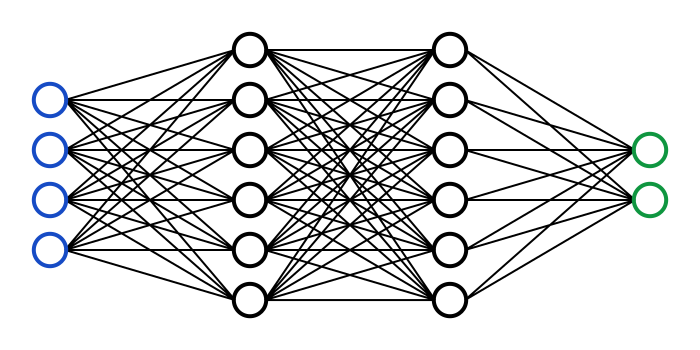
\includegraphics[scale=0.5]{images/neuralnetwork.png}
    \centering
    \caption{A graphical representation of a fully-connected feed-forward multi-layered perceptron network.}
    \label{fig:neuralnetwork}
\end{figure}

To more mathematical describe how the network operates: Data in nodes $x_i$ of the previous layer is transformed/scaled by the weight of the edge $w_{ji}$ and offset by the bias $b_i$ of the next node.
Therefore the data $h_i$ of the next layer is given by:

\begin{equation}
    h_i = \sum_j{w_{ji}x_j} + b_j
\end{equation}

In matrix notation, the transformation for all nodes in a layer can be expressed in one formula, where for any given layer index $l$: $h_l$ is the data values, $W_l$ is a matrix of edge weights and $b_l$ is the bias (offset).

\begin{equation}
    h_{l+1} = W_lh_l + b_l
\end{equation}

Therefore a simple NN can be thought of as a repeated process of matrix-vector multiplications and vector additions.
Such an algorithm produces behavior that can be adjusted to many given problems, as long as the size of the network is adequate to the problem at hand.
The size of the network is usually determined by the number of learnable parameters, which are adjusted by the number of layers and their width.
Because MLPs only contain linear operations, their behavior is limited to modeling linear relationships.
This is a limitation that might still work well for very simple applications, more difficult problems may require more dynamic behavior.
To produce such Activation Layers are used and built into the network.

\subsection{Activation Layers}

In order to introduce non-linear behavior to the network, Activation Layers are applied to the data at selected layers as it is transformed and fed through the network.
Activation Layers are differentiable but typically non-linear functions, we will see in section \ref{optimizers} why they have to be differentiable.
% The choice of what kind of Activation Layers to use and how many lies with the network architect.

One widely used activation functions and also most relevant to this work are ReLU (Rectified Linear Unit) and LeakyReLU (Leaky Rectified Linear Unit).
They both consist of two parts, in the positive domain both are $f(x) = x$, but in the negative domain ReLU is $f(x) = 0$ and LeakyReLU is $f(x) = c * x$ where c is a parameter.

\begin{figure}[h]
    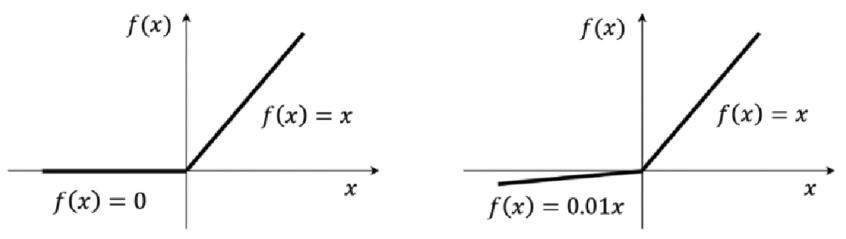
\includegraphics[scale=1]{images/relu.png}
    \centering
    \caption{Plots of ReLU (left) and LeakyReLU (right) activation functions.}
    \label{fig:activationfunctions}
\end{figure}

\subsection{Supervised Learning}
\label{supervised-learning}

The type of NNs relevant to this work all learn by the principle of Supervised Learning.
Supervised Learning is the process of learning based on labeled sample data (training data), which is fed into the network.
Since training data has to be created before a model can be trained, this limits the applicability to problems, where a solution (truth) is known beforehand.
For example, the best next chess move is not easily decided on, therefore this approach would not be feasible for a chess problem.

By comparing the network's results with the truth during training a Loss is calculated by a Loss Function (see section \ref{loss}).
This loss represents the 'wrongness' of the network.
It is then used by the Optimizer (see section \ref{optimizers}), an algorithm that adjusts the weights and biases (parameters) of the network in such a way, that the loss decreases and therefore the results are getting closer to the truth each iteration.
This is accomplished by calculating the gradient of the loss function in the current state via backpropagation.
This way of adjusting the parameters based on the loss is only possible because all the operations the network performs are differentiable and the gradient of the 'loss landscape' (n-dimensional space) can be calculated.

\subsection{Loss Functions}
\label{loss}

There are many Loss Functions a network architect can choose from.
Depending on the characteristics of the function, the network's learning behavior changes, as we understand in the following sections.

In general, a loss function produces a minimal value if the output of the network $y_i$ matches the expected truth $\hat{y}_i$.

\subsubsection*{Mean Absolute Error / L1 Loss}

L1 Loss or Mean Absolute Error Loss returns the absolute difference between the network output and the truth, which is averaged over the individual training batch.

\begin{equation}
    MAE = \frac{\sum_i^n |y_i - \hat{y}_i|}{n}
\end{equation}

\subsubsection*{Mean Squared Error / L2 Loss}

L2 Loss or Mean Squared Error Loss behaves differently to L1 Loss in the way that it does not calculate the absolute difference, but instead squares the difference of each value before averaging.

\begin{equation}
    MSE = \frac{\sum_i^n (y_i - \hat{y}_i)^2}{n}
\end{equation}

\begin{figure}[h]
    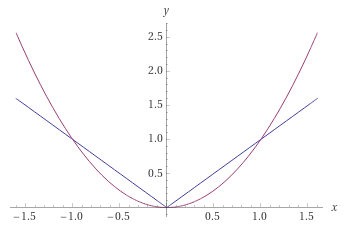
\includegraphics[scale=0.5]{images/l1l2loss.png}
    \centering
    \caption{A comparison of L1 and L2 Loss.}
\end{figure}

As seen in the figure above, the behavior of L1 is different when compared to L2.
This has consequences for the learning behavior of the network, in the case of $|y_i - \hat{y}_i| > 1$ L2 Loss has a greater value, which will cause the optimizer to change the parameters of the network more drastically than in the case of L1.
This can be an advantage or disadvantage depending on what you are interested in achieving and the scale of output data of your network.
Another advantage of MSE loss is the tangent and differentiable behavior around 0.
By having the gradient approach 0 near the origin this loss function ensures a 'homing in onto the minima' effect, which makes it harder for the optimizer to overshoot the minima.

\subsubsection*{Log-Cosh Loss}

Another popular loss function is the Log-Cosh Loss Function.
It combines the low gradient near 0 advantage of L2 Loss with linear loss behavior of L1 Loss.

\begin{equation}
    LC = \frac{\sum_i^n log(cosh(y_i - \hat{y}_i))}{n}
\end{equation}


\begin{figure}[h]
    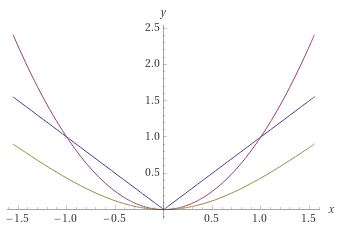
\includegraphics[scale=0.5]{images/l1l2logcoshloss.png}
    \centering
    \caption{A comparison of L1, L2, and Log-Cosh Loss.}
\end{figure}

\subsection{Optimizers}
\label{optimizers}

The task of an optimizer is, as its name states, to optimize a given function.
In our case, it optimizes/reduces the loss of the network by iteratively tweaking its parameters, which are initialized randomly.
The optimizer knows what parameter to adjust in which way by performing a stochastic gradient descent, it calculates the gradient based on a subset (batch) of the training data.

It decides how to tune these parameters based on its underlying algorithm and optional hyperparameters.
Probably the most important hyperparameter is the learning rate, it is basically the step size, the amount the optimizer changes the network's parameters each iteration.
When the learning rate is too high, the optimizer traverses the loss landscape (see figure \ref{fig:loss-landscape}) too quickly, which may result in minima being skipped over.
A too low learning rate will result in the training loop taking much more time than necessary to find a minimum.
But even if it does, we can be much less certain that the found minimum is a global one, much less than if it had found it with a higher learning rate.
This is since an optimizer with a lower learning rate will traverse the loss much less than one with a higher learning rate.
As the choice of selecting a learning rate is non-trivial, one can apply a learning rate finder.
It runs the training loop with many different learning rates in order to find a value that converges quickly while keeping its divergence during training minimal.

\begin{figure}[h]
    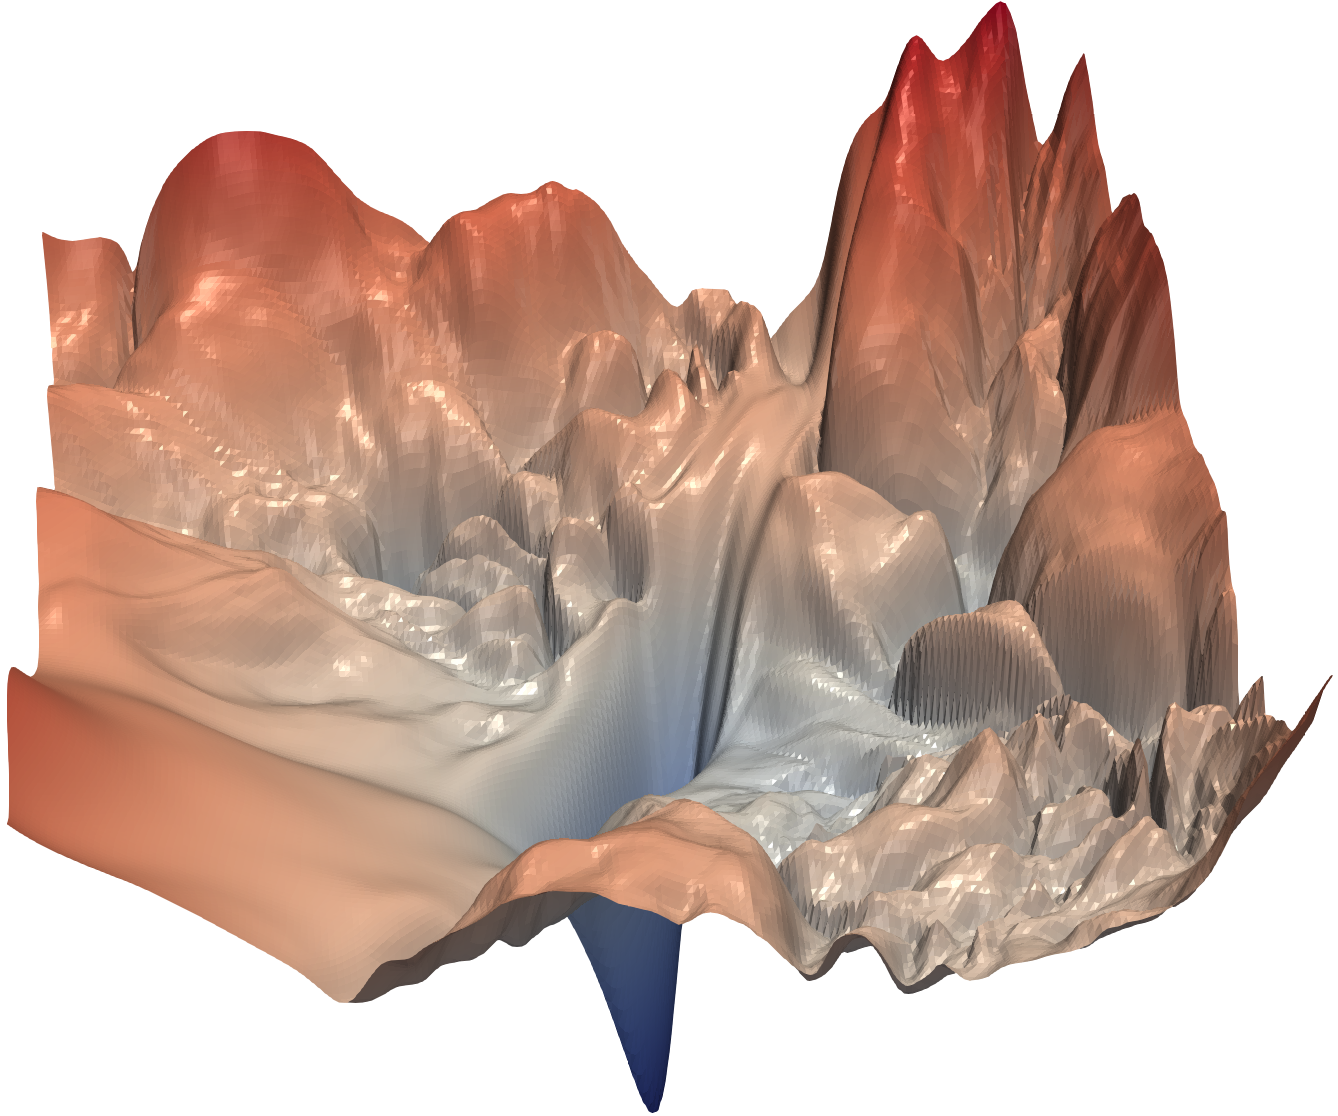
\includegraphics[scale=0.15]{images/loss-landscape.png}
    \centering
    \caption{A simplified 3D representation of the loss landscape of a complicated function.}
    \label{fig:loss-landscape}
\end{figure}

% \subsubsection*{Adam}

% Adam (Adaptive Moment Estimation) is one of the most popular optimizers, mainly due to its adaptive step size, which allows it to change the network's parameters more drastically when it is confident the loss landscape is smooth.
% This makes it a very versatile optimizer in many scenarios since it automatically adjusts its learning rate to speed up training.
% It starts off with the user-provided base learning rate but then assigns each parameter its learning rate which it adjusts dynamically.

\subsection{Overfitting and Early Stopping}

% Following the loss gradient 'downhill' does indeed reduce the loss observed each iteration.
% However since the loss does get smaller and smaller with each step, how would one know when to stop the training?
% One would easily believe that the lower our observed loss the better - so just keep on training, right?

\subsubsection*{Overfitting}

When a large enough neural network trains on a dataset for long enough, it will eventually reach a perfect loss on the training data since it will adjust its parameter to match/model the dataset at hand.
Its predictions get increasingly closer to the expected values as the loss is decreased over time.
However, once the trained model is evaluated on another dataset, it is apparent, that the network has adjusted itself to the specifics of the dataset it has been trained on.
Thus it fails to generalize to the underlying truth because picked up on the noise in the training data.
% When the model is evaluated on another dataset its performance is much worse than on the data it has been trained on.
This is a problem that has to be solved because the network is expected to perform its best even on new data it has never seen before.

\begin{figure}[h]
    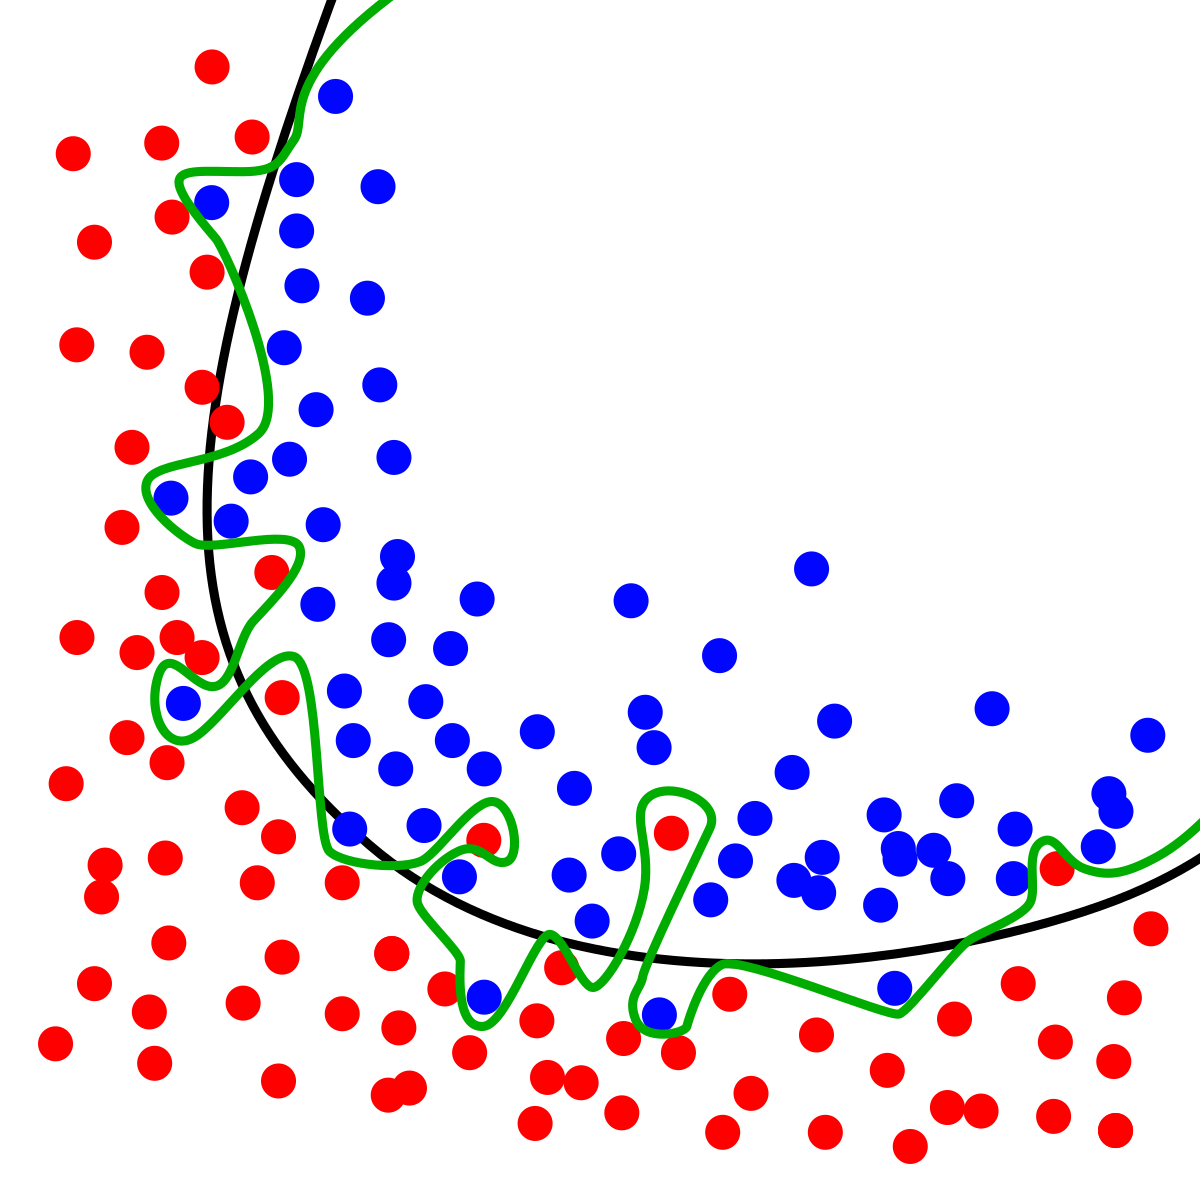
\includegraphics[scale=0.15]{images/Overfitting.svg.png}
    \centering
    \caption{A graphical representation of Overfitting. In this case, the network adjusts to the details of the noisy training data (red and blue points) instead of picking up on the general black division of the colors \cite{wiki:Overfitting}.}
    \label{fig:overfitting}
\end{figure}

\subsubsection*{Early Stopping}
\label{earlystopping}

Early Stopping aims to stop the training process at the point where the network performs its best on not yet seen data.
The point at which it has not yet picked up on the specifics (noise) of the training data.
As vaguely introduces in the previous section, the whole dataset that is available for training is usually split into three parts: Training, Validation, and Test Datasets.

The Training Dataset is fed to the network to calculate gradients (backpropagate) in order to descend in the loss landscape.
The Validation Dataset on the other hand is only fed to the network to evaluate its performance (calculate its loss), but never to backpropagate.
Finally, after training, the Test Dataset is used to evaluate the network's final performance, it is used separately from the Validation Dataset to suppress any influence of it being used as the indicator of when to stop training.

More accurately, after each Epoch (the network has seen all of the Training Data exactly once) it calculates and logs the loss of the network on the Validation Dataset.
First, the loss on the training data, as well as the loss on the validation data, both decrease together (see figure \ref{fig:earlystopping}).
After a certain number of Epochs, the validation loss will increase again due to the network overfitting to the training data.
When this happens Early Stopping will continue training for a set number of epochs (patience) before stopping the training and rolling the parameters of the network back to the state it was when the Validation Loss was minimal.
This results in an optimally performing network, that generalizes as well as possible to the underlying problem.

\begin{figure}[h]
    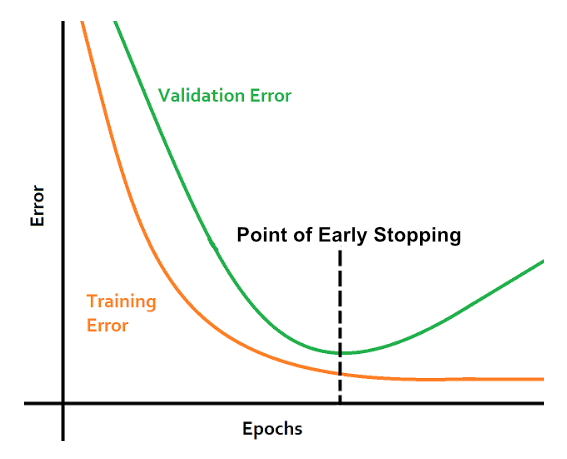
\includegraphics[scale=0.4]{images/early-stopping.png}
    \centering
    \caption{A simple plot of the training and validation loss during training.}
    \label{fig:earlystopping}
\end{figure}

\subsection{Learning Rate Schedulers}

In order to speed up training, but also to improve the accuracy of the optimizer hitting the/a minima in the loss landscape learning rate schedulers are used.
They change the learning rate of the optimizer during the training process.
Initially, usually, the learning rate is set high, to allow the initially completely unaware network to start learning quickly.
This has the disadvantage that the network most likely skips over (many) minima (as previously in section \ref{optimizers}).
After a few epochs, the learning rate scheduler usually decreased the learning rate gradually, as to allow the optimizer to reach the minima without overshooting it or oscillating around it.
The use of a learning rate scheduler generally results in quicker training with better results.

% \begin{figure}[h]
%     \includegraphics[scale=0.3]{images/learning-rate-schedulers.png}
%     \centering
%     \caption{An illustration of good and bad learning rates.}
%     \label{fig:learning-rate-schedulars}
% \end{figure}

\subsection{Weighted Loss}
\label{weighted-loss}

Usually, the loss for all data records is handled equally.
But in some cases, it makes sense to apply a weight to all losses individually.
A common case for weighing losses in classification (binary network output) is when the given training dataset is imbalanced.
An imbalanced dataset contains records which a majority classifies as one of the two possible binary values.
This would/will lead the network to prefer this value over the other, this behavior is known as bias.
Bias is generally undesirable since it discriminates against the minority and therefore yields poor performance in identifying records of the minority class.

To solve this problem one can cut a percentage of the majority from the training dataset in order to produce a balanced dataset in which both classes appear equally often, this approach is called undersampling.
This can be problematic when the majority outnumbers the minority by a very large factor, since then many individual records are lost when balancing out the dataset.
With way, fewer cases to learn from the network may struggle to fully understand all cases.
When facing such an issue one can apply weighted loss to the training data.
Instead of cutting a percentage from the majority class, a lower weight is applied to all records of the majority class.
The weights are picked in such a way that the sum of all losses of the majority class equals the sum of all losses of the minority class.
This way the network can learn from all available records without getting biased towards the majority.

\subsection{Graph Neural Networks}
\label{gnns}

Since the DOMs of IceCube are located in an irregular hexagonal grid pattern, the use of MLPs is unsuitable.
MLPs view all edges as equals, therefore assuming an equal distribution of nodes and equal distance between them, like a cubic grid pattern.
Because this is not the case for IceCube, a more flexible model is required.

Graphs are a set of nodes and edges, where each node can be connected to all other nodes (even themselves) via edges.
Edges can be either one-directional or undirected, allowing two nodes to influence another, in contrast to the feed-forward rule of MLPs.
Since not all nodes have to be connected, this allows for much more freedom when building a graph.
The decision of which nodes are connected via edges is an important one, it heavily influences how the network behaves and models relationships like social or molecular connections because edges are often actively used when computing on graphs.
Each node can hold multiple values (its features), instead of solely containing a singular value.

In the case of IceCube, each DOM taking part in an event is modeled as a node.
These nodes are then connected via edges, decided on by the k-nearest-neighbors algorithm (kNN).
It connects each node with the (in this case) 8 nearest neighbors in space \cite{rasmus-master}.

This generated graph is then interpreted by a Graph Neural Network, which takes the graph as its input.
In contrast to the ''one shape fits all'' approach of MLPs (or similar), this allows GNNs to adjust much better to different shapes of input data.
GNNs have proven great performance in various fields, such as social modeling at e.g. Facebook \cite{facebook}, interpretation and classifications of point clouds objects, as well as protein folding predictions \cite{STROKACH2020402}.

% Expanding heavily based on MLPs, Graph Neural Networks (GNNs) allow much looser rules for the node connecting edges.
% Edges can be bidirectional, which means that the logic from before when the previous layer influences the next, is not valid anymore.
% Instead two or more nodes can influence one another through the bidirectional edges.
% Also the number of connections (edges) to each node can vary based on the connection logic (e.g. k nearest neighbors) and does not necessarily have to be constant over all nodes.

\begin{figure}[h]
    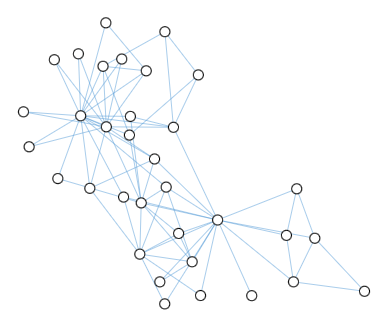
\includegraphics[scale=0.6]{images/graphneuralnetwork.png}
    \centering
    \caption{A graphical representation of a graph.}
    \label{fig:graphneuralnetwork}
\end{figure}

Let's now look into how GNNs operate on the input graph in more detail.

A GNN operates on a given graph by performing several (arbitrary amount) iterations of Message Passing.
During Message Passing each node sends ''messages'' to its neighbors iteratively updating their data based on the messages received.
Messages are typically based on the data the sending node holds, but can also contain other information like the number of edges.
Therefore messages are usually of the shape of the data contained in the node, but like layers can change the width in MLPs, the shape of messages is not fixed.
Each node combines the messages it receives, this aggregation logic could be taking the maximum, minimum, average, median, or any other sort of combining, as long as it is permutation invariant.
Permutation invariance is required since a graph does not hold information about the ordering of edges and therefore received messages.
Lastly, an update function generates the new data for each node, based on its old data and the aggregated messages.
The shape of data can change between iterations, based on the choice of message passing, aggregation, and update functions.

As the data contained in the graph has the shape $\texttt{Number of Nodes} \times \texttt{Number of Features}$, in order to produce a prediction vector (or singular value) this shape has to be reduced.
To achieve this the data of all nodes is aggregated by using a similar function as for the aggregation of messages.
Such functions can also be used in combination, as \texttt{dynedge}, the GNN used in this work, implements its node aggregation layer.
Finally the shape $\texttt{1} \times \texttt{Number of Features}$ is reduced again to the shape $\texttt{1} \times \texttt{Number of Output Variables}$, usually by the use of a MLP.

\subsubsection*{EdgeConv}

The GNN used in this work makes use of the \texttt{EdgeConv} convolutional layer \cite{1801.07829}.
\texttt{EdgeConv} was designed in order to make neural networks able to learn on graph point clouds, classifying or identifying objects based on their point cloud.
\texttt{EdgeConv} incorporates local neighborhood information into its message passing, allowing for the network to learn about the geometrical structure by analyzing each point in relationship with its neighborhood.

\begin{figure}[h]
    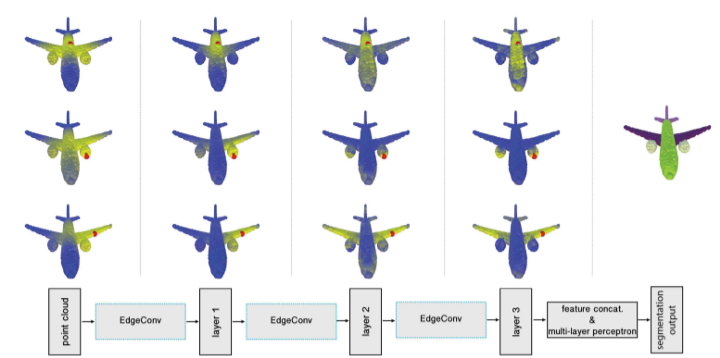
\includegraphics[width=\textwidth]{images/edgeconv.png}
    \centering
    \caption{An example application of EdgeConv \cite{1801.07829}.}
    \label{fig:edgeconv}
\end{figure}


\section{Icedata}
\label{icedata}

This section describes the IceCube ice model data and the process of preparing (reading, converting, interpolating) it for supervised learning.
% The properties of antarctic ice is not constant across the whole cubic kilometer of IceCube.
% The optical properties vary noticeably due to changing densities of the ice, but also because of impurities like dust.
In figure \ref{fig:icecube} the absorption and scattering is visualized, giving an overview of how the ice changes vertically.

The project SPICE \cite{1301.5361} measured the ice properties (icedata) and organized it into layers (ice of equal properties) indexed by depth.
Measurements were taken along 6 strings every \SI{10}{m} vertically.
The recorded values are not constant horizontally, therefore the layers are (slightly) tilted.
This tilt also varies across depth, which will complicate the interpolation process (section \ref{interpolation}).

Interpolation of the data is required because the position of each DOM must be associated with the ice properties of the layer it resides in.
Also, the \SI{10}{m} granularity of the data makes interpolation between them sensible.
The result of this interpolation process is visualized in figure \ref{fig:features_2d}.

\begin{figure}[h]
    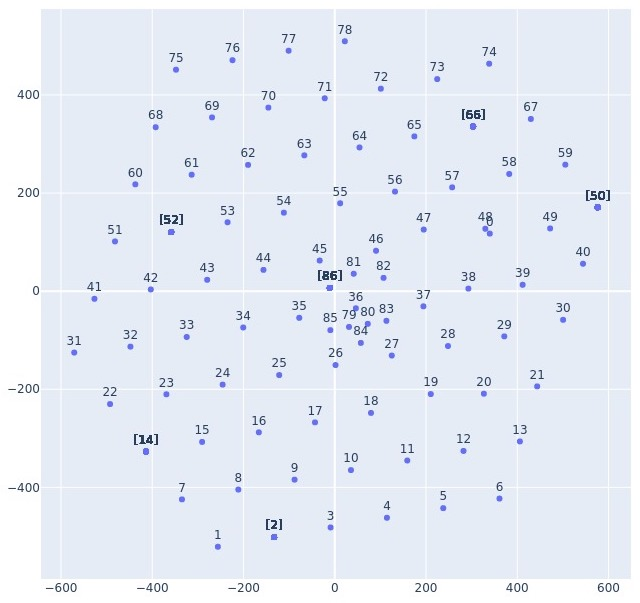
\includegraphics[scale=0.5]{images/string_overview.jpg}
    \centering
    \caption{An overview of where SPICE measurements have been taken. Strings, where measurements have been made, are marked with square brackets.}
    \label{fig:string_overview}
\end{figure}

\subsection{Coordinate Systems}
\label{coordinates}

Within IceCube there exist multiple types of coordinate systems which are commonly used \cite{coordinates-icecube}.
This section will outline the differences between the ones relevant to this work and provide conversions used when working with the icedata.

\subsubsection*{IceCube Coordinates}

Most of IceCube uses the IceCube coordinate system which has its origin \SI{1948.07}{m} below the surface, its $z$-coordinate will be called $z_{IceCube}$ and grows positive upwards.

\subsubsection*{SPICE Indexation}

The Spice dataset is organized and labeled by depth, which is 0 at the surface of the ice and grows positive downwards.
We will call this $z$-coordinate $z_{Depth}$ or simply Depth \cite{1301.5361}.

\subsubsection*{Global Coordinates}

The $z$-coordinate we will be working with (and converting the other coordinates into) is $z_{Global}$, a coordinate system that has its origin at the surface and grows upwards.
This definition results in the following conversions:

\begin{equation}
    z_{Global} = -z_{Depth}
\end{equation}
\begin{equation}
    z_{Global} = z_{IceCube} - \SI{1948.07}{m}
\end{equation}

\subsection{Data files from SPICE}
\label{files}

The data from SPICE comes in space-/tab-separated-values format and are read by using the Python \texttt{pandas} library.
For example, the file \texttt{tilt.par} is read like so:

\begin{verbatim}
import pandas as pd

df_tilt_par = pd.read_csv('tilt.par', sep=' ', names=['string_no', 'dist_sw_225'])
\end{verbatim}

\subsubsection*{icemodel.dat}

This file contains the ice properties listed below.
As loosely described above, the data is indexed by depth, which identifies the layer the row of data is related to.
The columns of data contained in this file stem from the ice model from \cite{1301.5361} and \cite{icemodel}:

\begin{itemize}
    \item \texttt{depth}: depth below surface (used as layer identifier)
    \item \texttt{be(400)}: scattering at wavelength of 400nm
    \item \texttt{adust(400)}: absorption at wavelength of 400nm
    \item \texttt{dT}: temperature delta (vs. value at \SI{1730}{m})
    \item \texttt{k1}: anisotropy coefficient (parallel to the axis)
    \item \texttt{k2}: anisotropy coefficient (perpendicular to the axis)
          % \item \texttt{Abc}: TODO:
\end{itemize}

\begin{center}
    \begin{tabular}{ |c||c|c|c|c|c|c| }
        \hline
        Depth & be(400) & adust(400) & dT & k1 & k2 \\
        \hline
    \end{tabular}
\end{center}


\subsubsection*{tilt.par}

This file describes where the ice layer tilt offsets are measured at.
This means that the file contains a horizontal (xy) description of where the offsets are located.
\texttt{SW\_255} is the horizontal distance in the SouthWest (225deg) direction with its origin located at string 86.

% Due to the natural relationship between string number and its location the data is redundant and only \texttt{SW\_255} will be used from now on.

\begin{itemize}
    \item \texttt{string\_no}: string number
    \item \texttt{sw\_225}: distance [m] into the south-west direction (\SI{225}{^\circ}) direction
\end{itemize}

\begin{center}
    \begin{tabular}{ |c|c| }
        \hline
        String & SW\_225  \\
        \hline
        50     & -531.419 \\
        66     & -454.882 \\
        86     & 0        \\
        52     & 165.202  \\
        2      & 445.477  \\
        14     & 520.77   \\
        \hline
    \end{tabular}
\end{center}

\subsubsection*{tilt.dat}

This file describes how much each layer of ice is tilted at the locations specified in \texttt{tilt.par} relative to the flat assumption.
It holds the 6 offset values at all depths.
Together with the locations from above, it will be used to build a model of tilted layers.

\begin{center}
    \begin{tabular}{ |c||c|c|c|c|c|c| }
        \hline
        Depth & Offset 50 & Offset 66 & Offset 86 & Offset 52 & Offset 2 & Offset 14 \\
        \hline
    \end{tabular}
\end{center}

\subsection{Interpolation}
\label{interpolation}

As discussed in section \ref{icedata}, the layer tilt is not constant across depth, therefore the process of assigning a layer to an arbitrary point is non-trivial.
This is especially evident for the bottom-most layers, whose proximity to the bedrock gives them a curved shape, as seen in figure \ref{fig:layers_2d}.
Not only do the layers have to be interpolated over the horizontal axis, but also the icedata has to be interpolated vertically between the layers.
This process and all decisions/assumptions made are described in this section.

Since the layers are described at the locations defined in \texttt{tilt.par}, we use its z-southwest coordinate system.
More specifically we use $z_{Global}$ as the y-axis and distance in the southwest direction as the x-axis with string 86 as the origin.
Onward we will use the function \texttt{sw\_225} to calculate the sw-coordinate of any given point.

\begin{verbatim}
import numpy as np

SW_225 = np.array([-1, -1]) / np.sqrt(2)  # normalized direction vector
ORIGIN = XY_STRING[86]                    # string 86 is zero of `tilt.dat`

def sw_225(xy):
    return np.dot(xy - ORIGIN, SW_225)
\end{verbatim}

\subsubsection{Layers}

% \subsubsection*{Overview}

First, a function/algorithm is required to decide on what layer a given point is located in, or more accurately, what layers a given point is located between.
To build such a function, we interpolate the measured layer tilt offsets across the sw-coordinate.
By adding/subtracting the layer depth to the interpolated offset we get the actual layer heights at any point.
Doing this for all positions, we get the resulting layers shown in figure \ref{fig:layers_2d}.

\subsubsection*{Extrapolation}

As is visible in figure \ref{fig:string_overview} strings 7 and 1 extend further into the southwest direction than string 14, the last string a measurement has been made for.
This is also the case with strings 74, 67, and 59, which extend past the last measured string in the negative southwest direction, string 50.
This makes the choice to extrapolate the layers in both directions necessary.

\subsubsection*{Quadratic Interpolation}

As the layer offset is measured at 6 points in the southwest direction, we have to interpolate these values.
A quadratic interpolation was chosen instead of linear interpolation.
This decision is clearly biased, but hopefully the better choice.
The reasoning is, that the layers of ice are most likely not spikey/angled at the points of measurement, but rather smoothly changing their angle.
Therefore a quadratic interpolation will provide for more even and flowy layers, instead of spikey, undifferentiable layers.

\subsubsection*{Continued Layers}

Strangely the last layer contained in \texttt{tilt.dat} is at a depth of \SI{2448.47}{m}, which is a few dozen meters above the lowest DOMs.
Though the data contained in \texttt{icemodel.dat} extends all the way to a depth of \SI{2798.47}{m}.
To incorporate this existing data, the decision was made to simply copy the shape of the lowest layer 7 times.
This allows for an interpolation that respects the given icedata while hopefully being as close to the actual shape of layers as possible.
These additional layers are visible in figure \ref{fig:layers_2d}.

\subsubsection*{Code}

The interpolation was done using the 1D interpolation function provided by the python library \texttt{scipy} \cite{scipy}.
The data used is stored in \texttt{df\_tilt\_par} and \texttt{df\_tilt\_dat}, which comes from the corresponding files described in \ref{files}.

Since \texttt{interpolation\_dzs} only interpolates the offsets, we create another function \texttt{interpolation\_zs}, which adds the z-coordinate of every layer to the offsets and converts between the Spice coordinates and the global coordinates (see \ref{coordinates}).
It will return an array of the heights of all layers at the location it is given \texttt{sw}.

\begin{verbatim}
from scipy.interpolate import interp1d

interpolation_dzs = interp1d(
    df_tilt_par.dist_sw_225.to_numpy(),  # positions where offsets were measured (6,)
    df_tilt_dat.iloc[:, 1:].to_numpy(),  # offsets = dzs (125, 6)
    kind='quadratic',
    axis=1,
    bounds_error=False,
    fill_value='extrapolate',
)

def interpolation_zs(sw): return -(df_tilt_dat.z - interpolation_dzs(sw))
\end{verbatim}

\begin{figure}[H]
    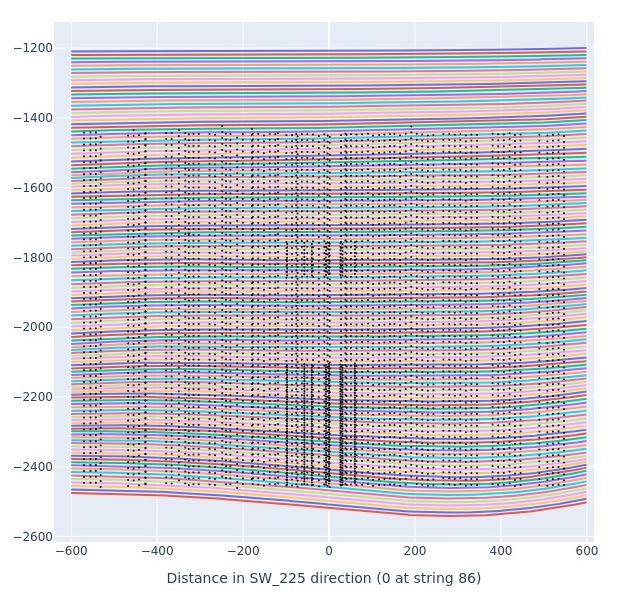
\includegraphics[scale=0.6]{images/layers_2d.jpg}
    \centering
    \caption{The interpolated ice layers (color) and all DOMs (black).}
    \label{fig:layers_2d}
\end{figure}

\subsubsection{Ice Properties}

To now compute the icedata at any point we first use \texttt{interpolation\_zs} designed above to get the heights of all layers at the location point of interest.
Then we do another interpolation, this time interpolating the icedata over the just calculated layers heights.
This gives us a function that will interpolate the icedata between the layer above and below the point of interest at a given height.

\subsubsection*{Quadratic Interpolation}

A quadratic interpolation was chosen for similar reasons as before for the layers.
It is intended to smooth over outliers in the data and make it less spikey.
Having a differentiable function to describe the properties is probably also a more correct approach.

\subsubsection*{Extrapolation}

If we had not previously continued the layers in \texttt{tilt.dat}, we would have to use extrapolation to calculate the icedata of the lowest DOMs.
But because we have extended the layers in order to contain all DOMs between them, extrapolation is not required here.

\subsubsection*{Code}

The functionality discussed above relies on the layer heights at the point of interest.
Therefore we run the function \texttt{interpolation\_zs} created before in order to get the layer heights.
We use use this data together with the icedata from \texttt{icemodel.dat} to build the second interpolation, again using the 1D interpolation function from \texttt{scipy} \cite{scipy}.

The function \texttt{interpolation\_features} will return a 2D array of icedata specific to the point of interest identified by its sw- and z-coordinate.

\begin{verbatim}
layer_zs_global = interpolation_zs(sw)

interpolation_features = interp1d(
    layer_zs_global,  # layer heights from before (125,)
    layer_features,   # icedata from icemodel.dat aligned with layers from tilt.dat (125, 6)
    kind='quadratic',
    axis=0,
    bounds_error=False,
    fill_value='extrapolate',
)
\end{verbatim}

\subsection{Lookup Table}

A lookup table containing pre-interpolated ice properties for all DOMs is created in order to minimize computational overhead during training.
So instead of interpolating the features on every occurrence during training, we precalculate the values for all DOMs beforehand.
To achieve this, we loop over all DOMs and their positions, calculate their sw-coordinate and then calculate their icedata.
The lookup table itself is implemented as a simple key-value store (Python dictionary), which uses the DOM locations (xyz) as its key and returns a 6 element array containing the icedata for that DOM.

\begin{figure}[H]
    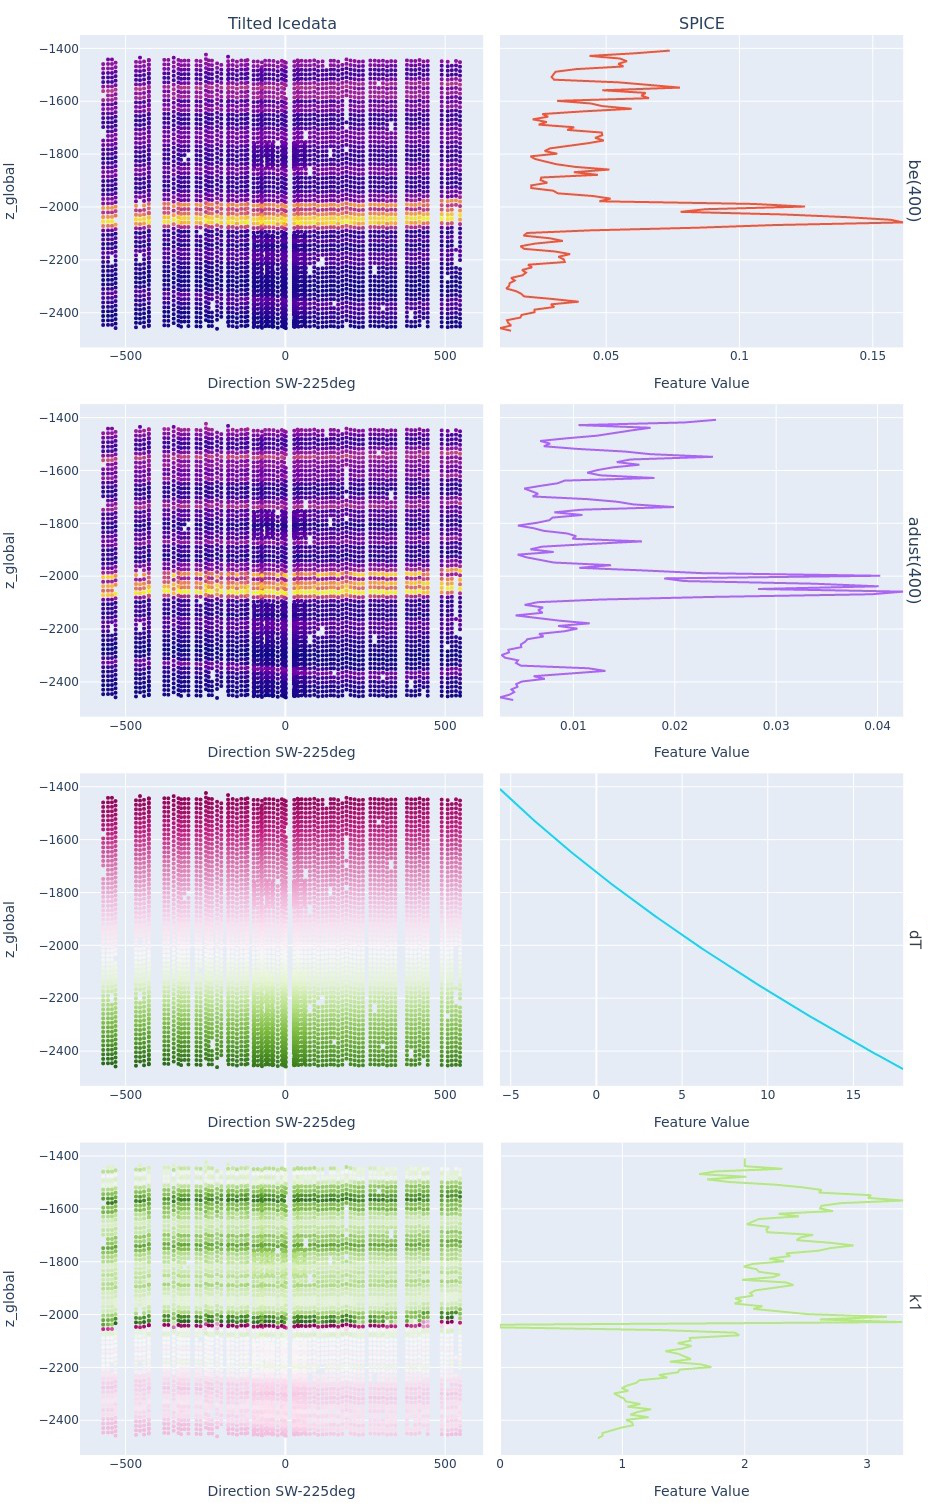
\includegraphics[scale=0.40]{images/feature_2d.jpg}
    \centering
    \caption{
        A visualization of icedata that has been interpolated to all DOM locations.
        On the left side, a projection of all DOMs onto the southwest axis is shown.
        The color of the dots relates to the interpolated feature value of each DOM.
        The tilt of ice layers is clearly visible, as obvious from figure \ref{fig:layers_2d} this is most prominently below \SI{-2000}{m}.
        On the right side, the raw feature value is plotted over height, this is the value that was used by the interpolation process described above.
    }
    \label{fig:features_2d}
\end{figure}

\section{The GNN \& Training Procedure}

\subsection{GraphNeT}
\label{graphnet}

\texttt{GraphNeT} \cite{graphnet} is a machine learning library that makes applying a Graph Neural Network to data from PMT-based neutrino telescopes (such as IceCube or KM3NeT) easy.
It is built on top of PyTorch \cite{torch}, one of the most popular open-source machine learning frameworks.
Its modular approach allows for easy use and customization, GraphNeT uses \texttt{PyTorch} as a basis and implements modules and adapters which interface with the IceCube data.
Because PyTorch itself does not implement the use of graphs, an additional library \texttt{PyTorch Geometric} \cite{torch-geometric} is used for the generation and learning on graphs.

As previously touched on in section \ref{gnns}, graphs are generated for each event with DOMs as nodes and edges created by the k-nearnest-neighbors algorithm.

\subsection{dynedge}

The most widely used GNN implemented in GraphNeT is \texttt{dynedge} \cite{2209.03042}.
It consists of five EdgeConv layers, the first layer operates on the graph generated by the k-nearest-neighbors algorithm with all nodes containing the unmodified DOM data from section \ref{variables}.
After the first layer, the number of features is increased, by being scaled up by an MLP.
The results of all five EdgeConv layers are then concatenated into an even wider shape.
Afterward, another MLP is applied, the data is aggregated and finally, a last final MLP brings the data into the output shape.

\begin{figure}[h]
    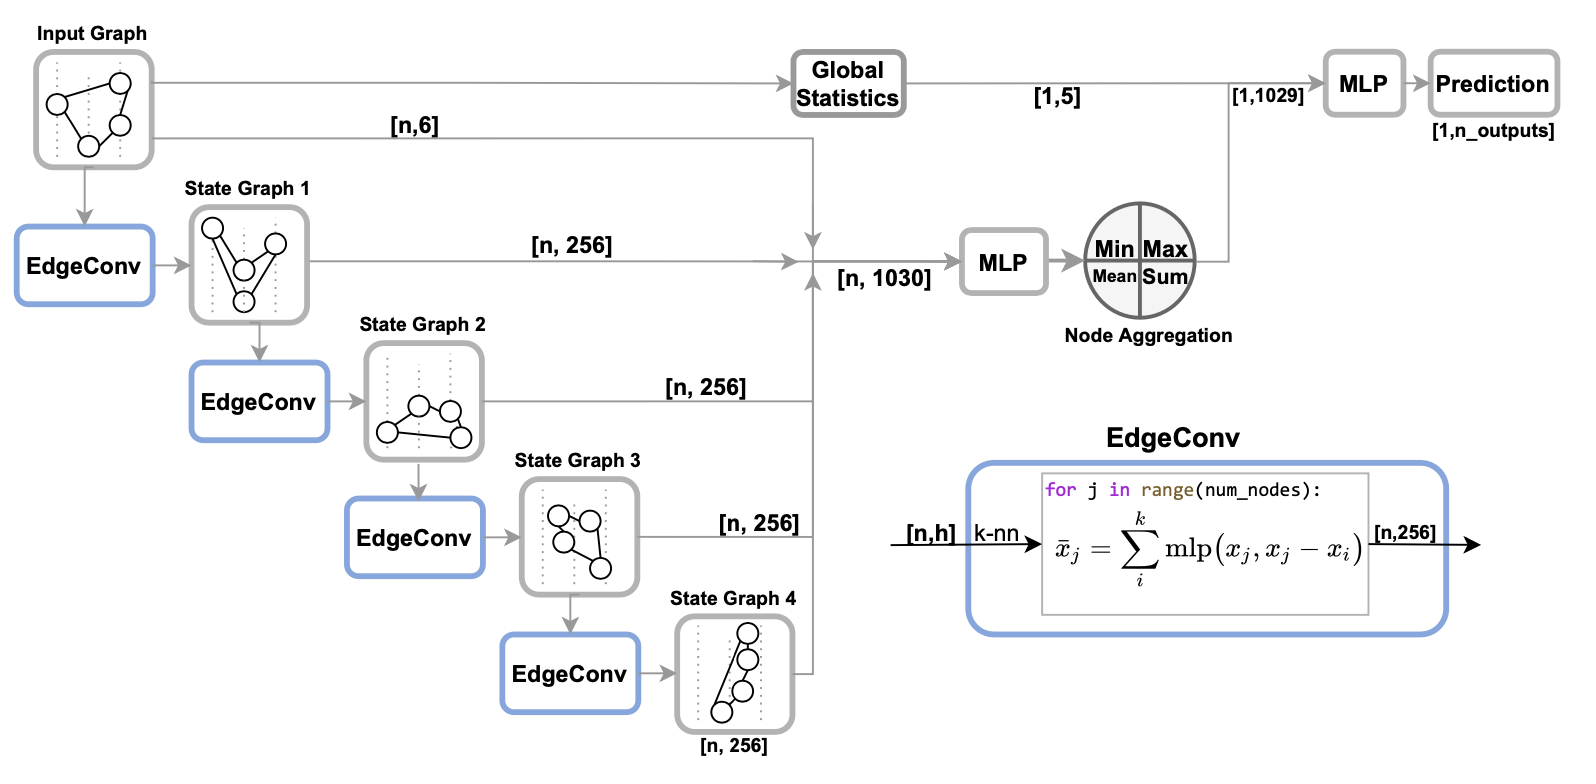
\includegraphics[width=\textwidth]{images/dynedge.png}
    \centering
    \caption{A diagram of the GNN model dynedge \cite{2209.03042}.}
    \label{fig:dynedge}
\end{figure}

\subsection{Inserting Icedata}

There exist several sensible approaches to inserting the icedata into training.
One could do calculations on each graph edge and calculate probabilities of absorption based on the absorption rate and distance and let this value influence message passing.
One could calculate optical distance based on the refractive index between any two DOMs and modify the k-nearest-neighbors algorithm to use it instead of real distance.
One could also weigh graph edges based on a combination of the values above.
For simplicity and in order to test whether the icedata gives any benefit to the network at all, it was decided to attach the local icedata to the features of each node.
That means that the feature variables from section \ref{variables} have been extended to also contain all ice properties from section \ref{icedata}.
As touched on before, a lookup table was generated before training and the code loading the data for each DOM was modified to look up icedata based on the DOMs position and attach that data to the node's features.

In order to reach a generally well-performing network, Early Stopping was utilized during the training process.
As the optimizer, the choice was made to use Adam, since it allows for quicker learning on average.
Especially in this case, because the addition of icedata will drastically and unpredictably complicate the loss landscape, Adam is a great choice, since it automatically adapts its learning rate in order to navigate the local loss landscape more appropriately.
In addition to Adam a piecewise linear Learning Rate Scheduler was used, which scales the learning rate of Adam from $\SI{e-5}{}$ in the beginning, to $\SI{e-3}{}$ after the first half epoch and then back down again to $\SI{e-5}{}$ after 50 epochs.
This allows Adam to get to know the loss landscape a bit better after starting out and improves its accuracy in hitting a minimum at the end.

\subsection{Applying Weighted Loss}

Since the majority of events happen in the energy interval from $0$ to $\SI{1.5}{log10 GeV}$ it is sensible to focus our attention on these events, because the performance of the network is largely influenced by this set of data.
In order to improve the performance of the network for these kinds of events, a weighted loss was created which flattens the density per energy within this interval, while providing an inverse decrease outside the upper limit of the interval.
Usage of this weighted loss will cause the network to treat these energies as equally important and not specialize in the energy with the highest density (see section \ref{weighted-loss}).

\begin{figure}[h]
    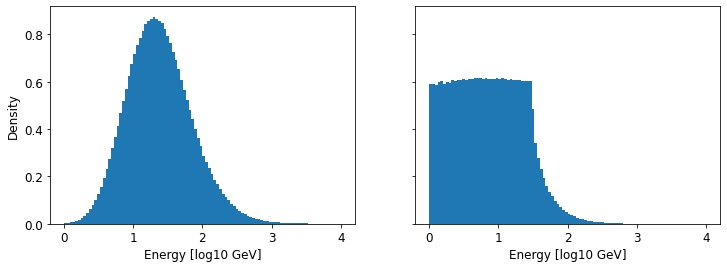
\includegraphics[width=\textwidth]{images/loss-weights.jpg}
    \centering
    \caption{A histogram comparing the standard (left) vs. weighted (right) event energy distribution.}
    \label{fig:weighted-loss}
\end{figure}


\section{Results \& Conclusions}

\subsection{Performance with Icedata}

After several runs of training with icedata attached to the features of nodes, it was clear that the performance of the network did not increase im comparison to the dynedge baseline.
The energy resolution produced by both version are plotted in figure \ref{fig:results-icedata} for comparison.
It is apparent that the average performance of both versions is nearly equal.
It can therefore be deduced that the additional information of the ice does not help the network understand the given problem any better than without.
One could assume that the network picks up on the different behavior of DOMs that is caused by the changing ice purely through the baseline feature variables.
Sadly understanding what a neural network thinks is thinking or understanding is not easily measurable, if at all.
Therefore this is simply a conclusion based on the fact that the additional knowledge does not seem necessary for the network.

Not mentioned before, it was also tried to transform the icedata with the use of \texttt{RobustScaler} and \texttt{QuantileTransformer} from the \texttt{scikit-learn} library \cite{scikit-learn}.
Although this was expected to improve the results at least a bit, did not yield any better performance.

\subsection{Performance with Icedata and Weighted Loss}

Applying a weighted loss to the events on the other hand did substantially increase the network's performance.
As visualized in figure \ref{fig:repeatability} the network's resolution improved noticeably in the areas where the weighted loss increased the attention of the network.
This is most apparent in the energy interval between $0$ and $\SI{0.75}{log10 GeV}$.
At high energies however, the accuracy became worse on average, because the attention of the network was reduced through the lower weight.
The weighted loss made the network perform better at the energies where the loss was increased and worse (on average) where the loss was decreased (see figure \ref{fig:weighted-loss}).
As is visible by looking at figure \ref{fig:repeatability} each training run with a weighted loss applied produced unreliable behavior at high energies.
This repeatability problem is more closely explored in the following section.
It is most interesting to see that although the performance decreased on average, some runs managed to score as good or better than the baseline, which nicely shows how the network's final state heavily depends on the initial randomly chosen parameters of the network.

\subsection{Repeatability}

One important insight, that was made and has to be held in mind when investigating and testing with several variants of neural networks, was reproducibility/repeatability.
As usually any neural network is initialized with random parameters before training, it is not guaranteed that the optimizer will find the same loss minimum each time.
This makes comparisons between different training runs more difficult, as became apparent in the previous section.
It was indeed observed, that the performance of different training runs containing icedata and a weighted loss, and therefore having a way more complicated loss landscape, varies much more than variants without a weighted loss (see figure \ref{fig:repeatability}).

\subsection{Neutrino Oscillation Contours}

With the improved accuracy in predicting energy, as well as other predictions of the network Pisa, a Monte Carlo-based data analysis tool, can fit a mathematical model of neutrino oscillations to our network's predictions.
The fit has uncertainties, but its \SI{90}{\%} confidence range can be visualized by a contour plot (see figure \ref{fig:contour}).
One can see that the baseline dynedge model improves about \SI{25}{\%} on pisa's performance in terms of area.
The model developed in this work clearly improves on this even further about equally as much.

% \newpage

\begin{figure}[h]
    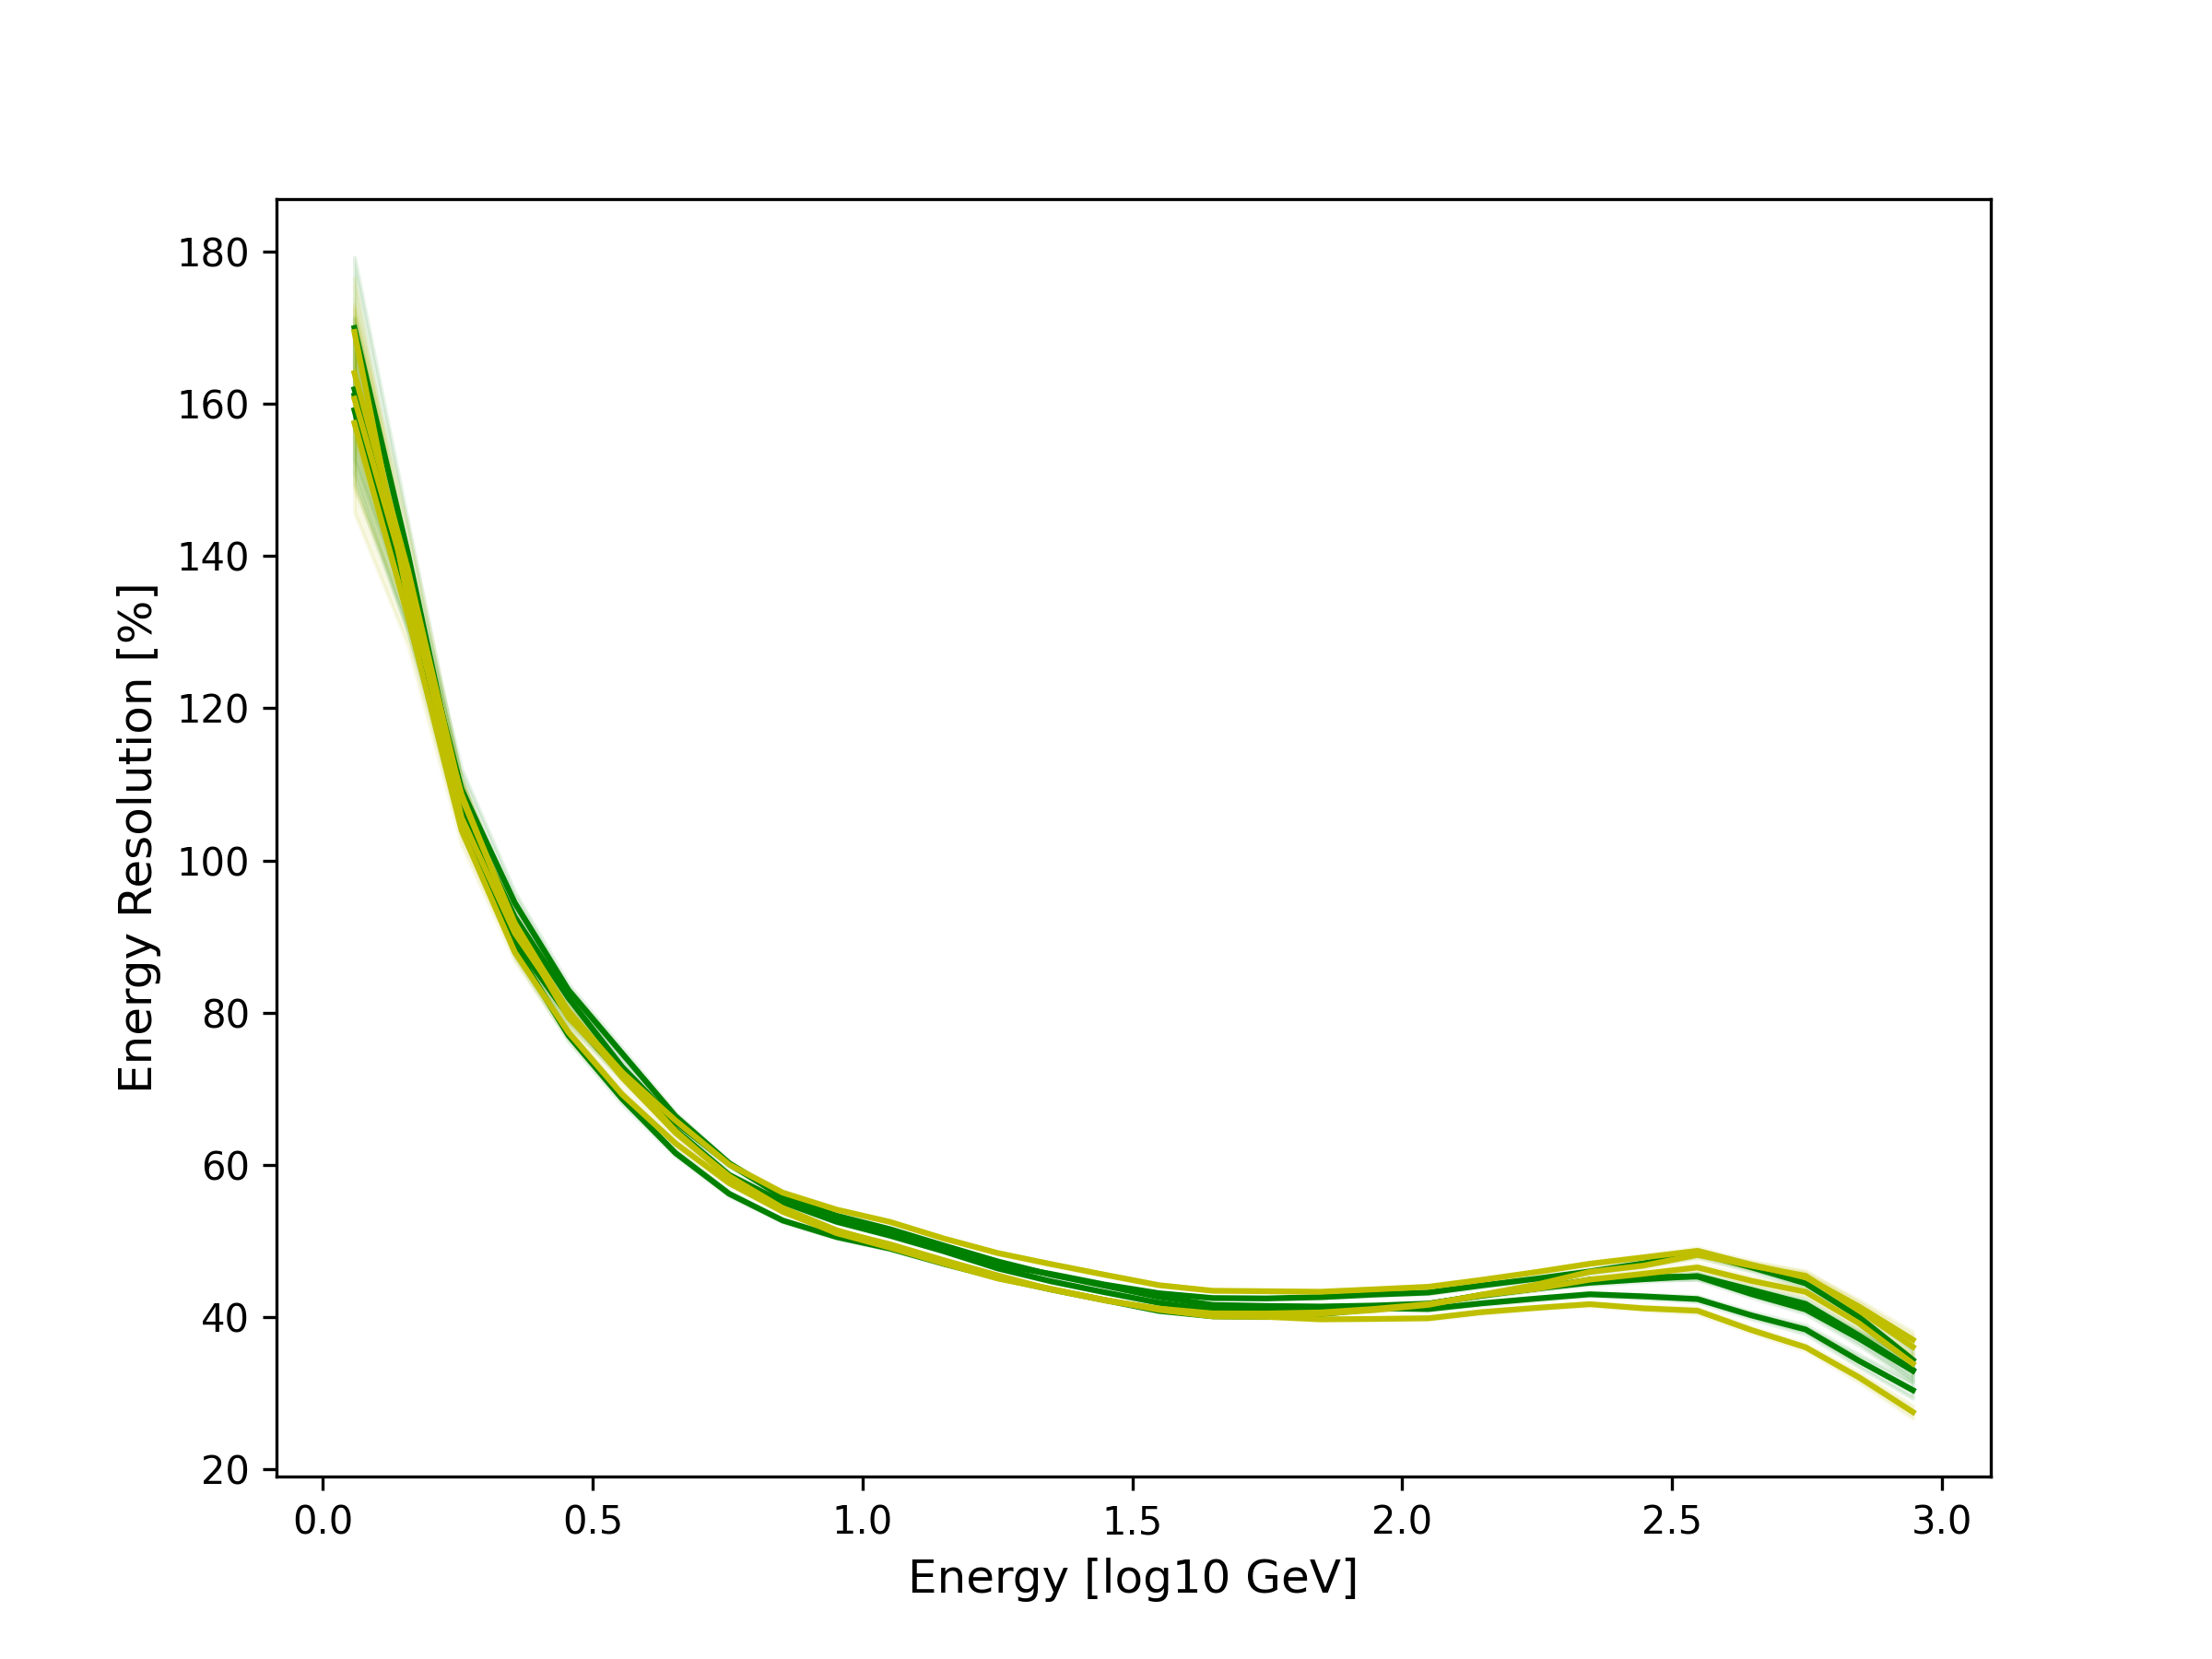
\includegraphics[scale=0.65]{images/results-icedata.png}
    \centering
    \caption{Energy resolution of different training runs. Runs with standard features are colored green, while runs with attached icedata are colored yellow.}
    \label{fig:results-icedata}
\end{figure}

\begin{figure}[H]
    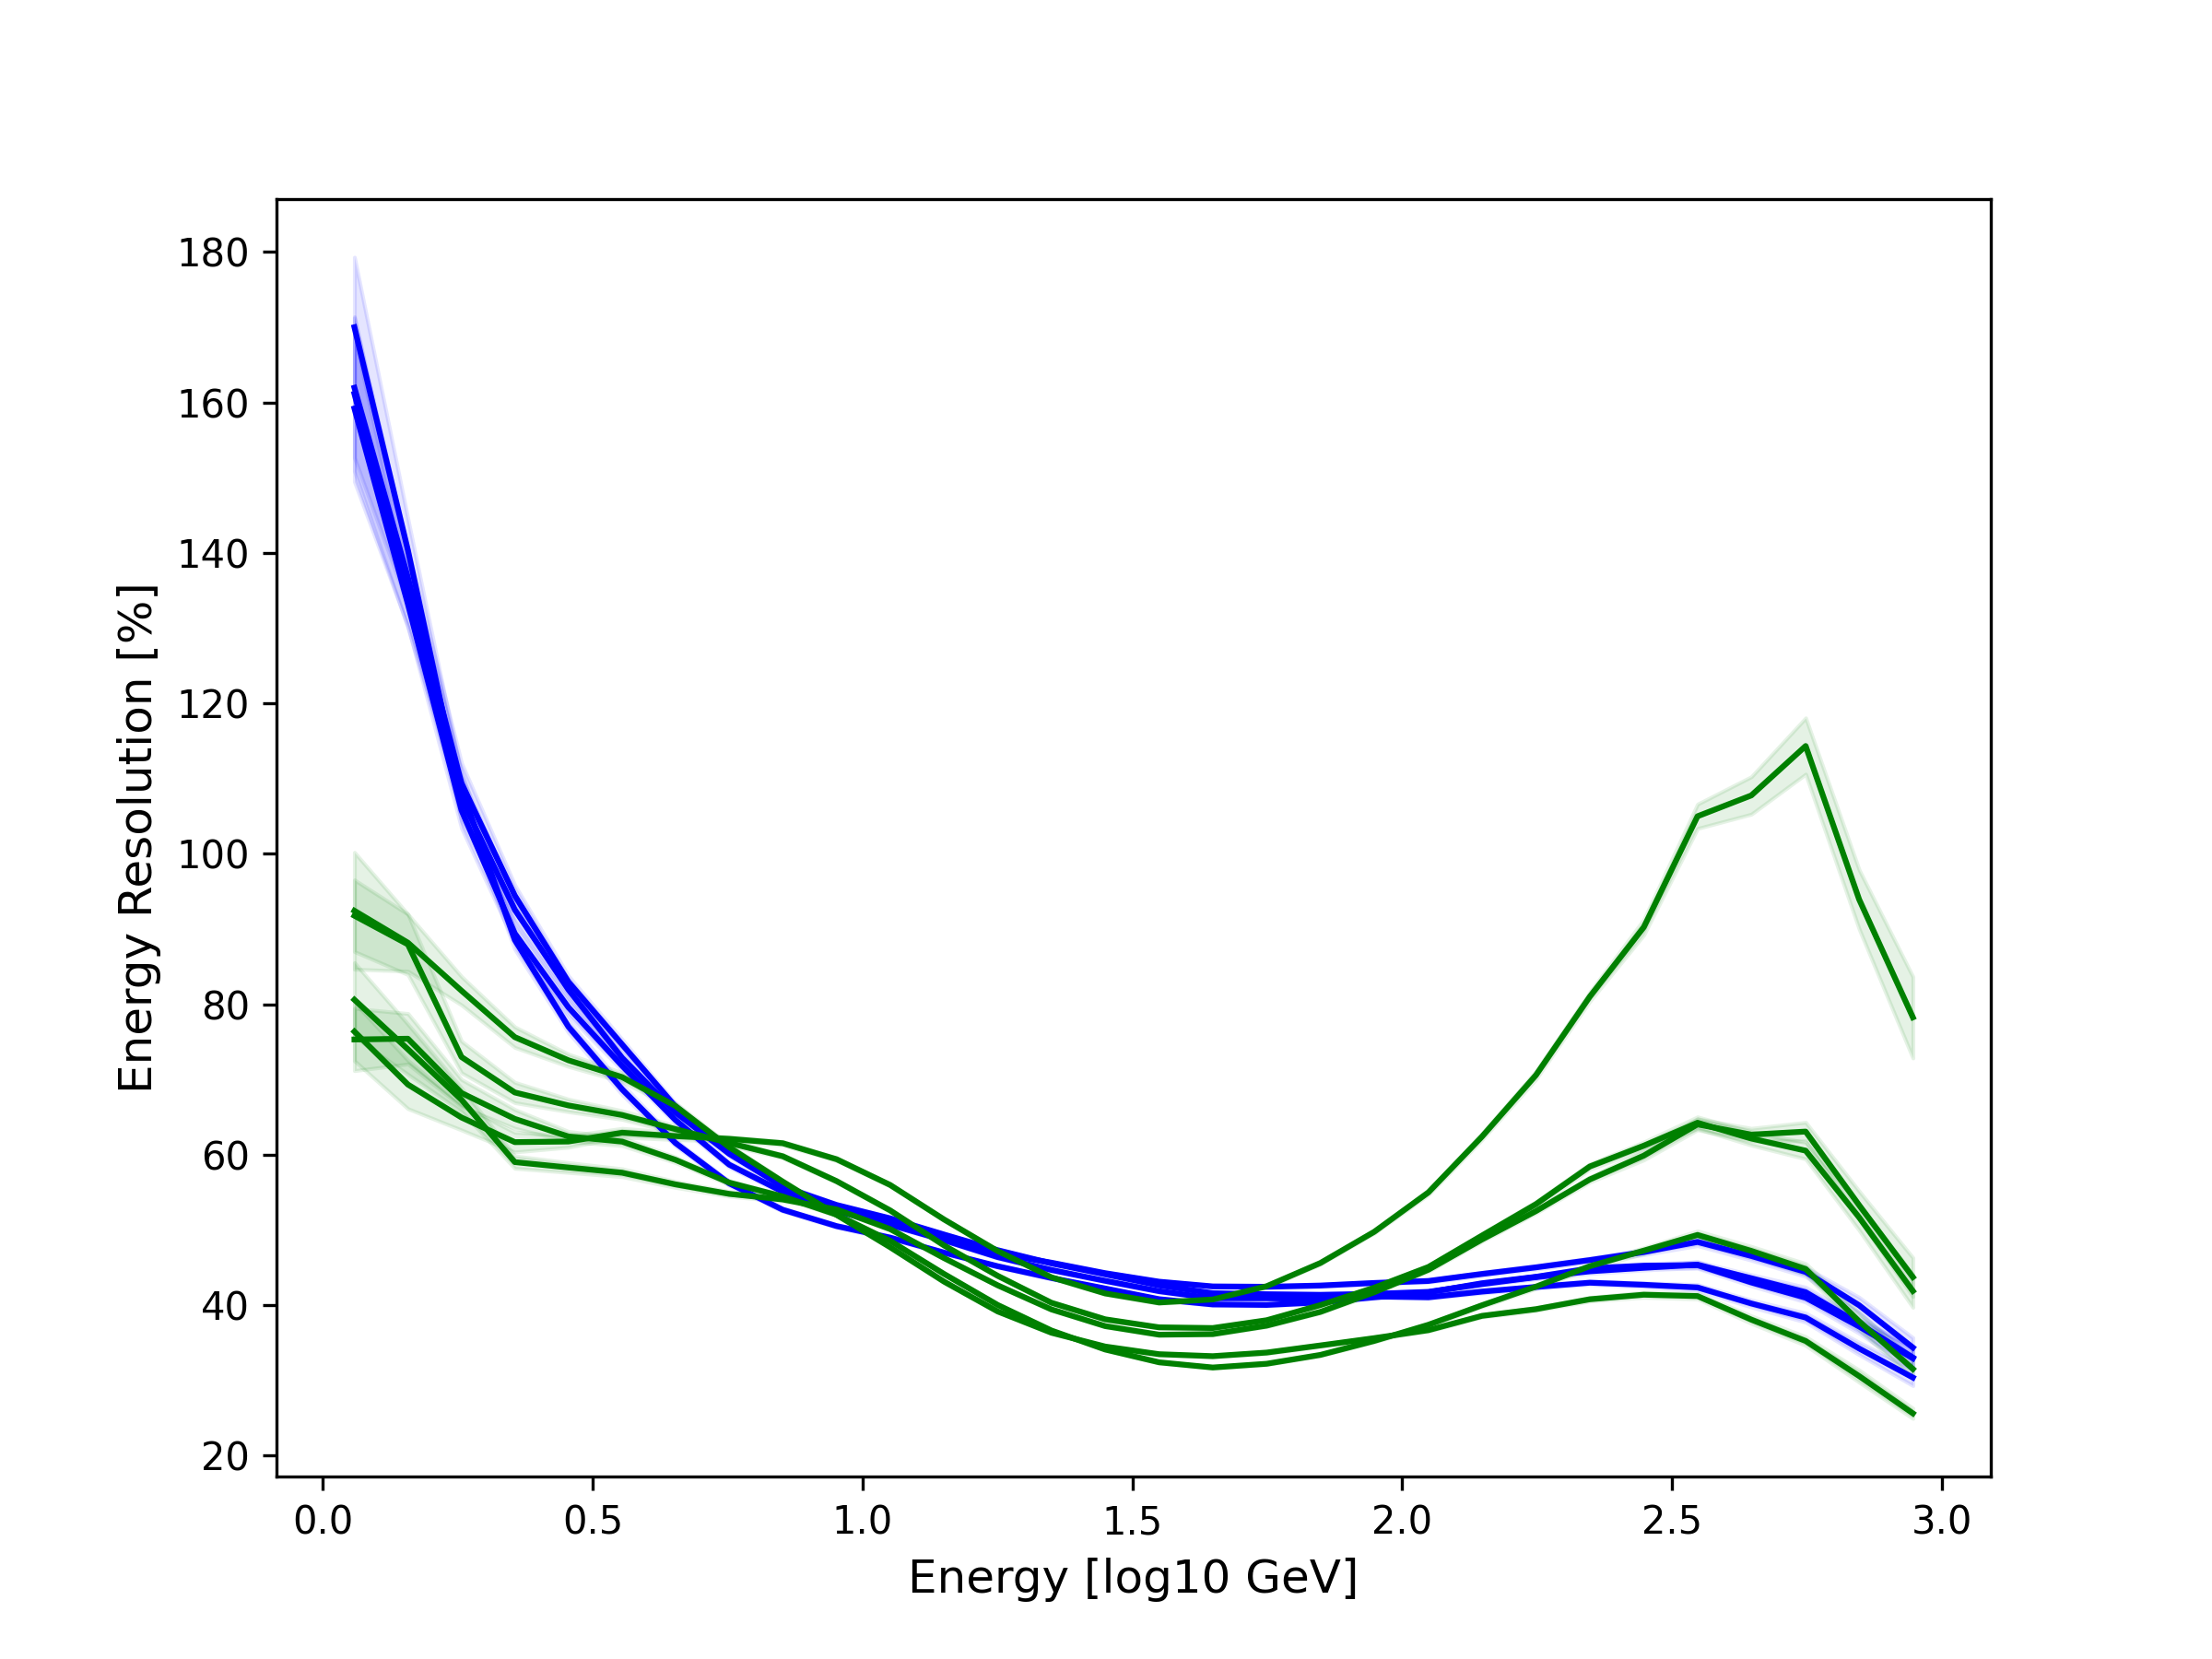
\includegraphics[scale=0.65]{images/repeatability.png}
    \centering
    \caption{Energy resolutions of different training runs. Runs with standard features are colored blue, while runs with attached icedata and weighted loss are colored green. All runs were trained with the same hyperparameters.}
    \label{fig:repeatability}
\end{figure}

\begin{figure}[H]
    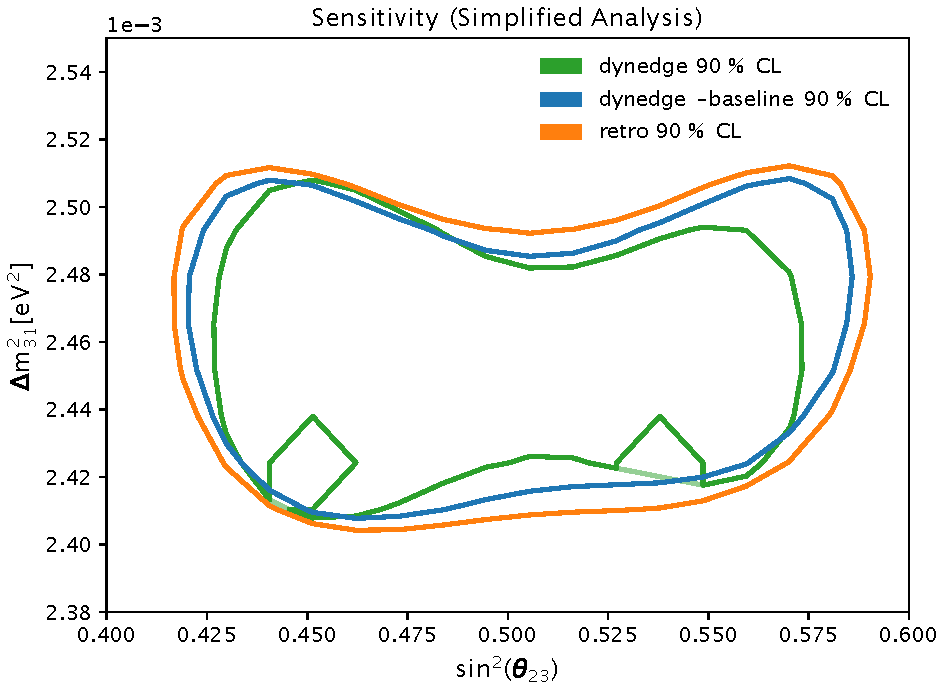
\includegraphics[scale=0.7]{images/2d_contour_test_fixed.pdf}
    \centering
    \caption{
        The neutrino oscillation fitting contours of dynedge with icedata and weighted loss vs. dynedge baseline and retro.
        (During fitting a convergence issue of the minimizer occurred, which is visible due to the two deformations of the green contour -
        One can expect the correct contours to behave like the blue and orange ones - This is illustrated by the green line with 50\% opacity)
    }
    \label{fig:contour}
\end{figure}

\newpage
\printbibliography

\end{document}
